\chapter{Figuren van de observaties}\label{sec:figobservaties}
Dit hoofdstuk bevat de testdata op een grafische manier voorgesteld. Dit is enkel een selectie van de figuren, al de data en figuren kunnen gevonden worden op \url{https://github.com/thuys/YCSB-Testdata}.  

%\begin{figure}[ht!] 
%	\centering
%	\subfigure[Normal Update]{\label{fig:consistentie-all-mongodb-normal} 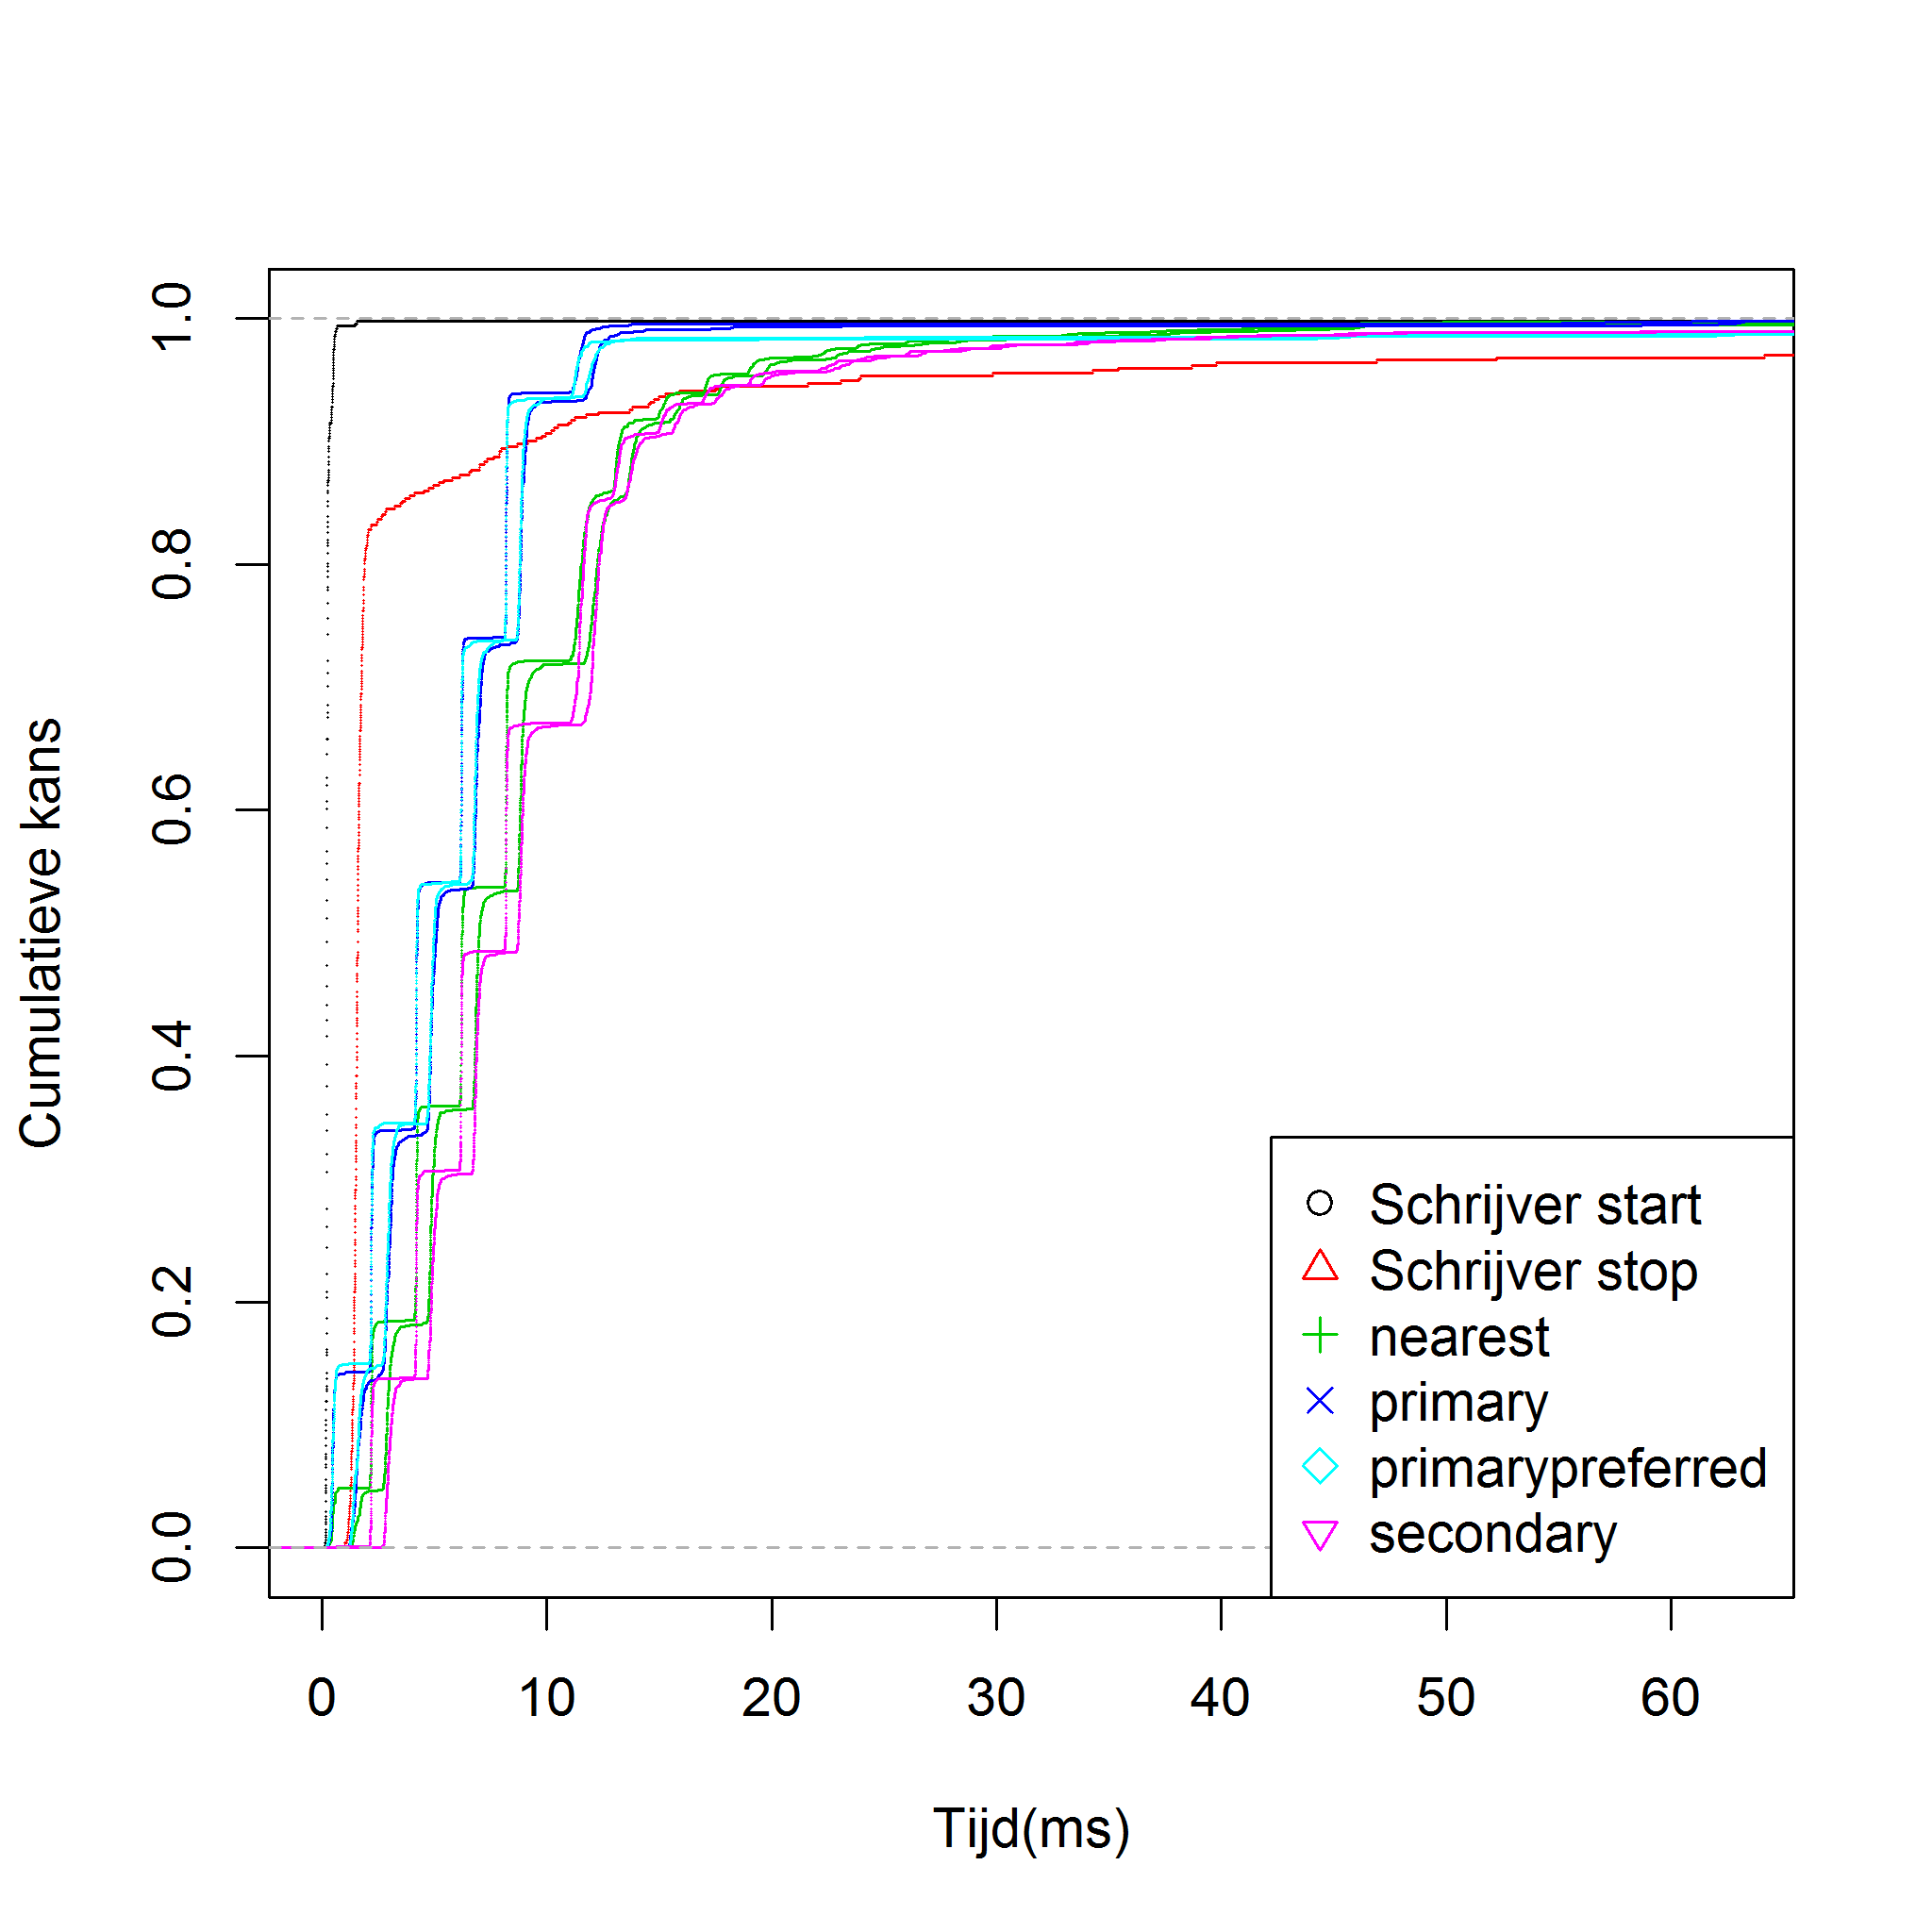
\includegraphics[width=.40\textwidth]{img/Observaties/MongoDB/ECDF-Reads-update-normal-all-2}}
%	\subfigure[Safe Update]{\label{fig:consistentie-all-mongodb-safe} 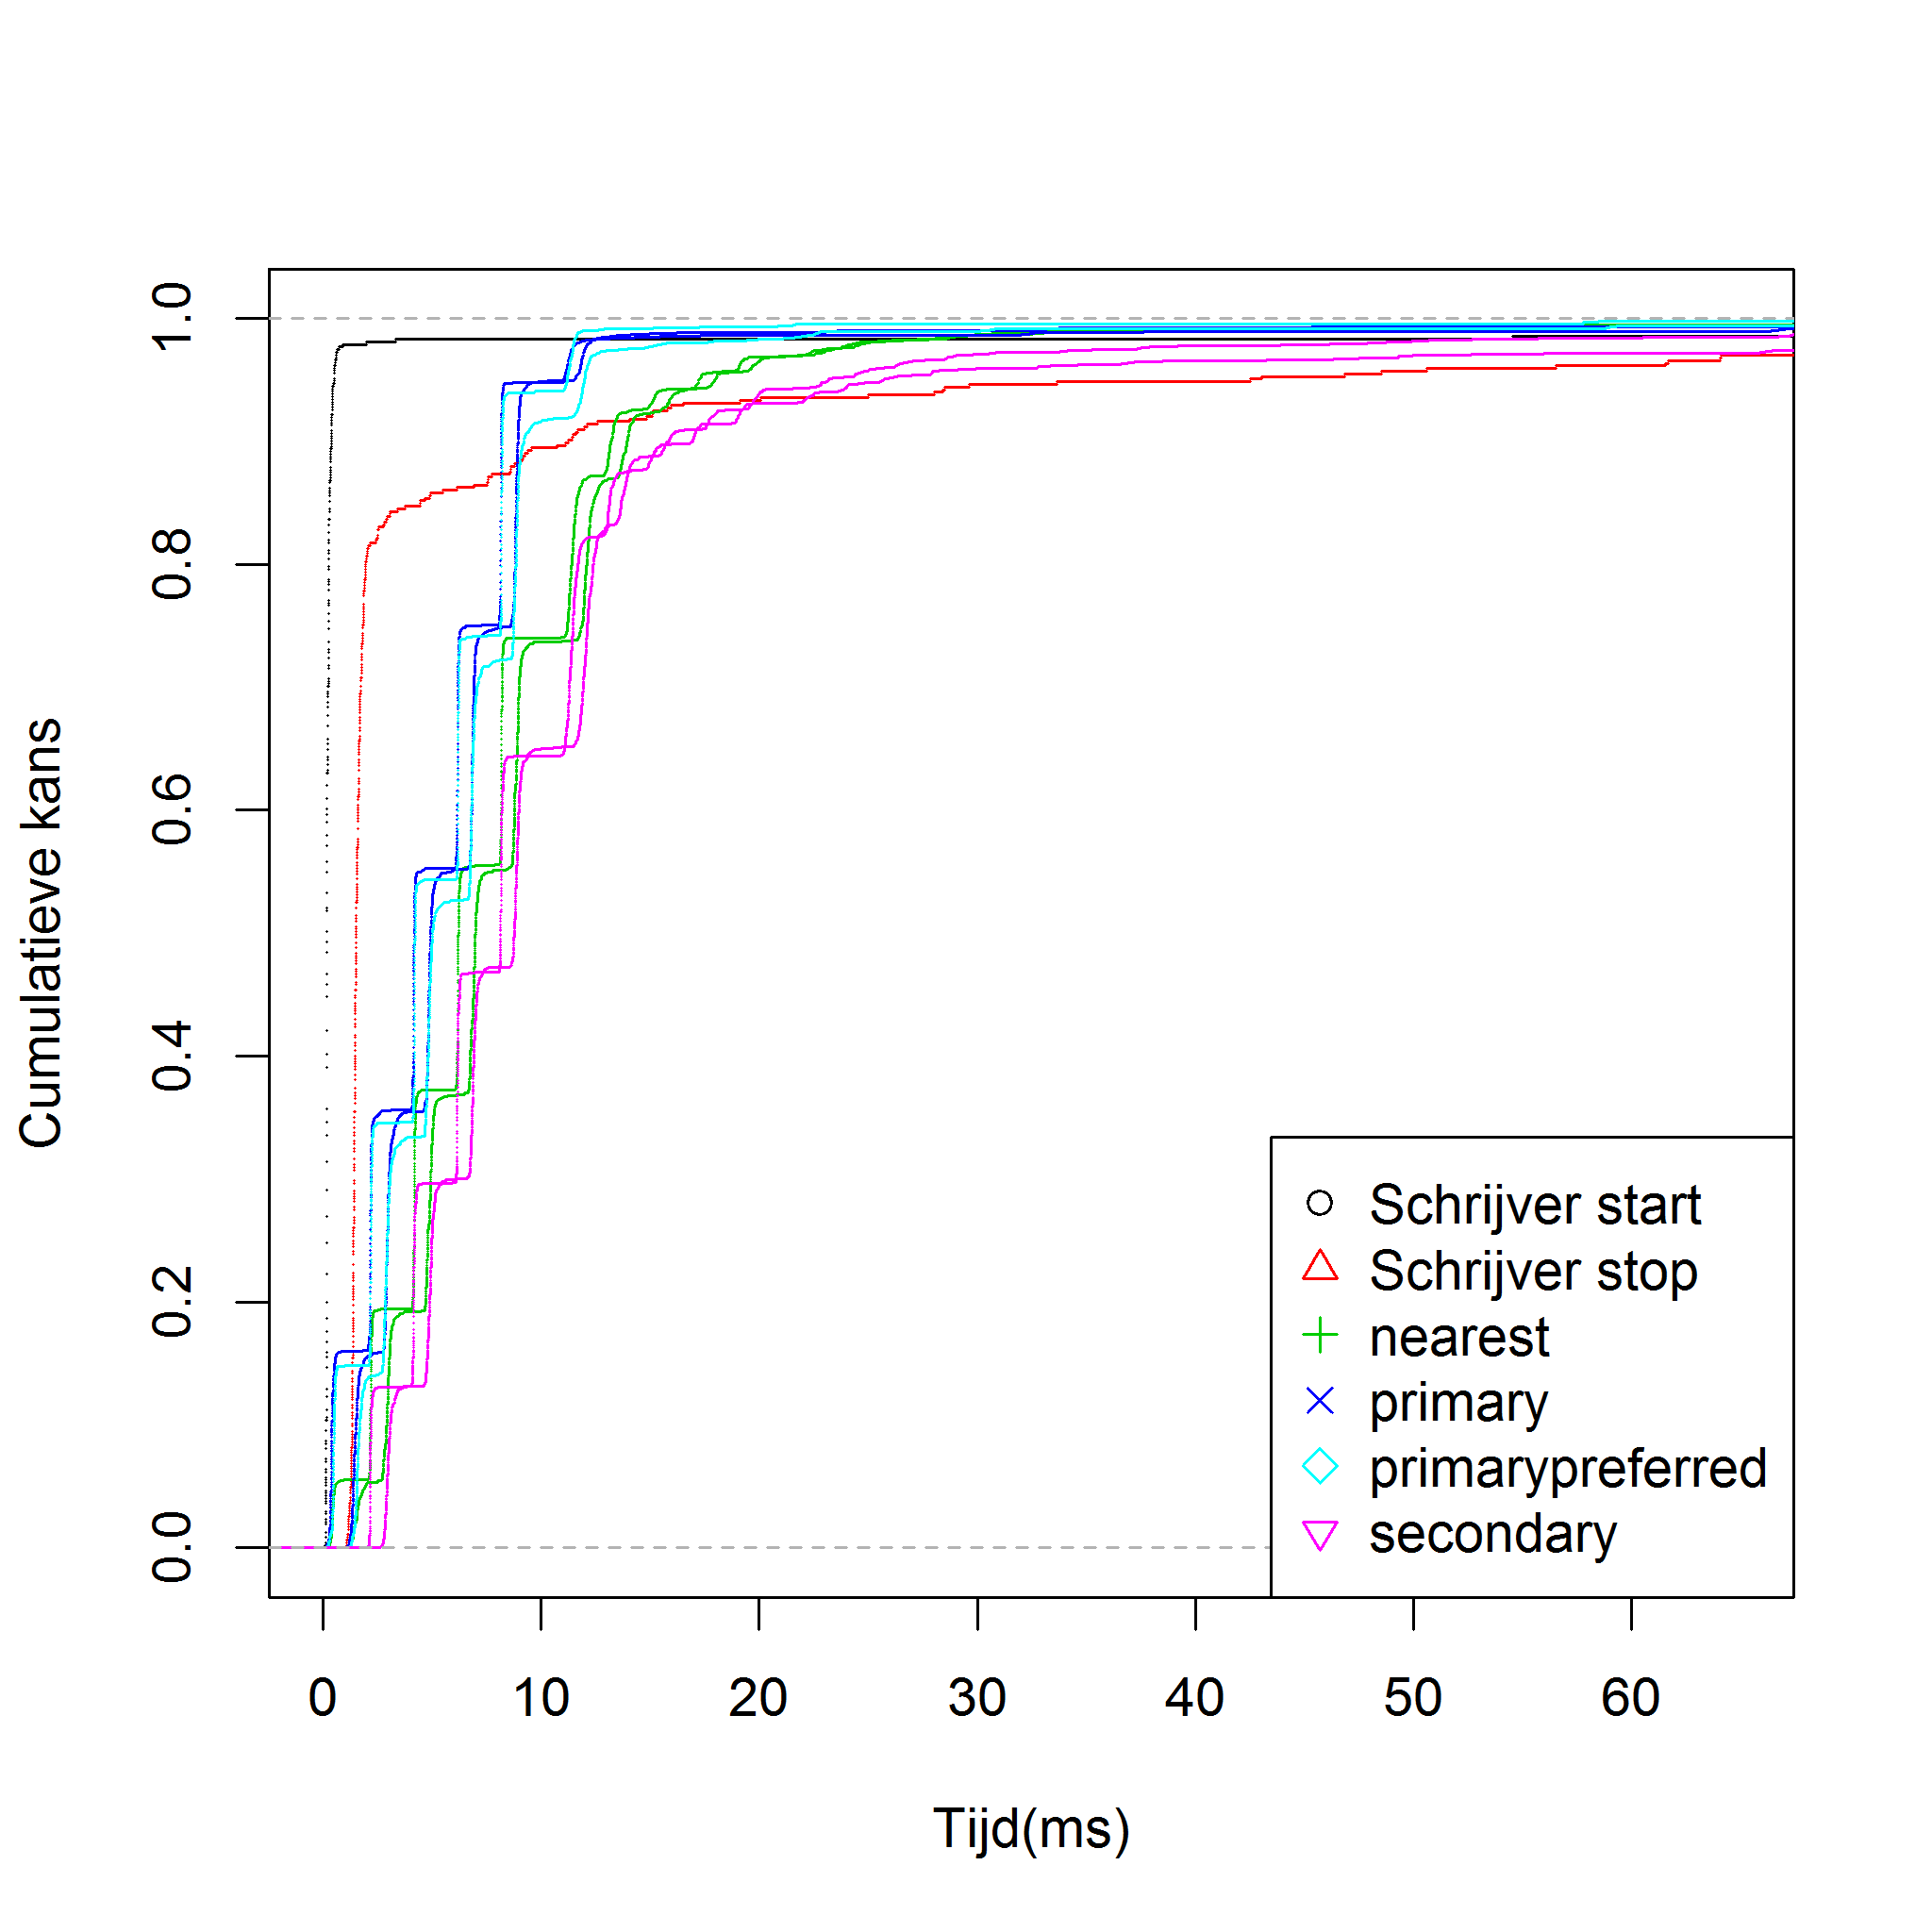
\includegraphics[width=.40\textwidth]{img/Observaties/MongoDB/ECDF-Reads-update-safe-all-2}}
%	\subfigure[Fsync Safe Update]{\label{fig:consistentie-all-mongodb-fsync} 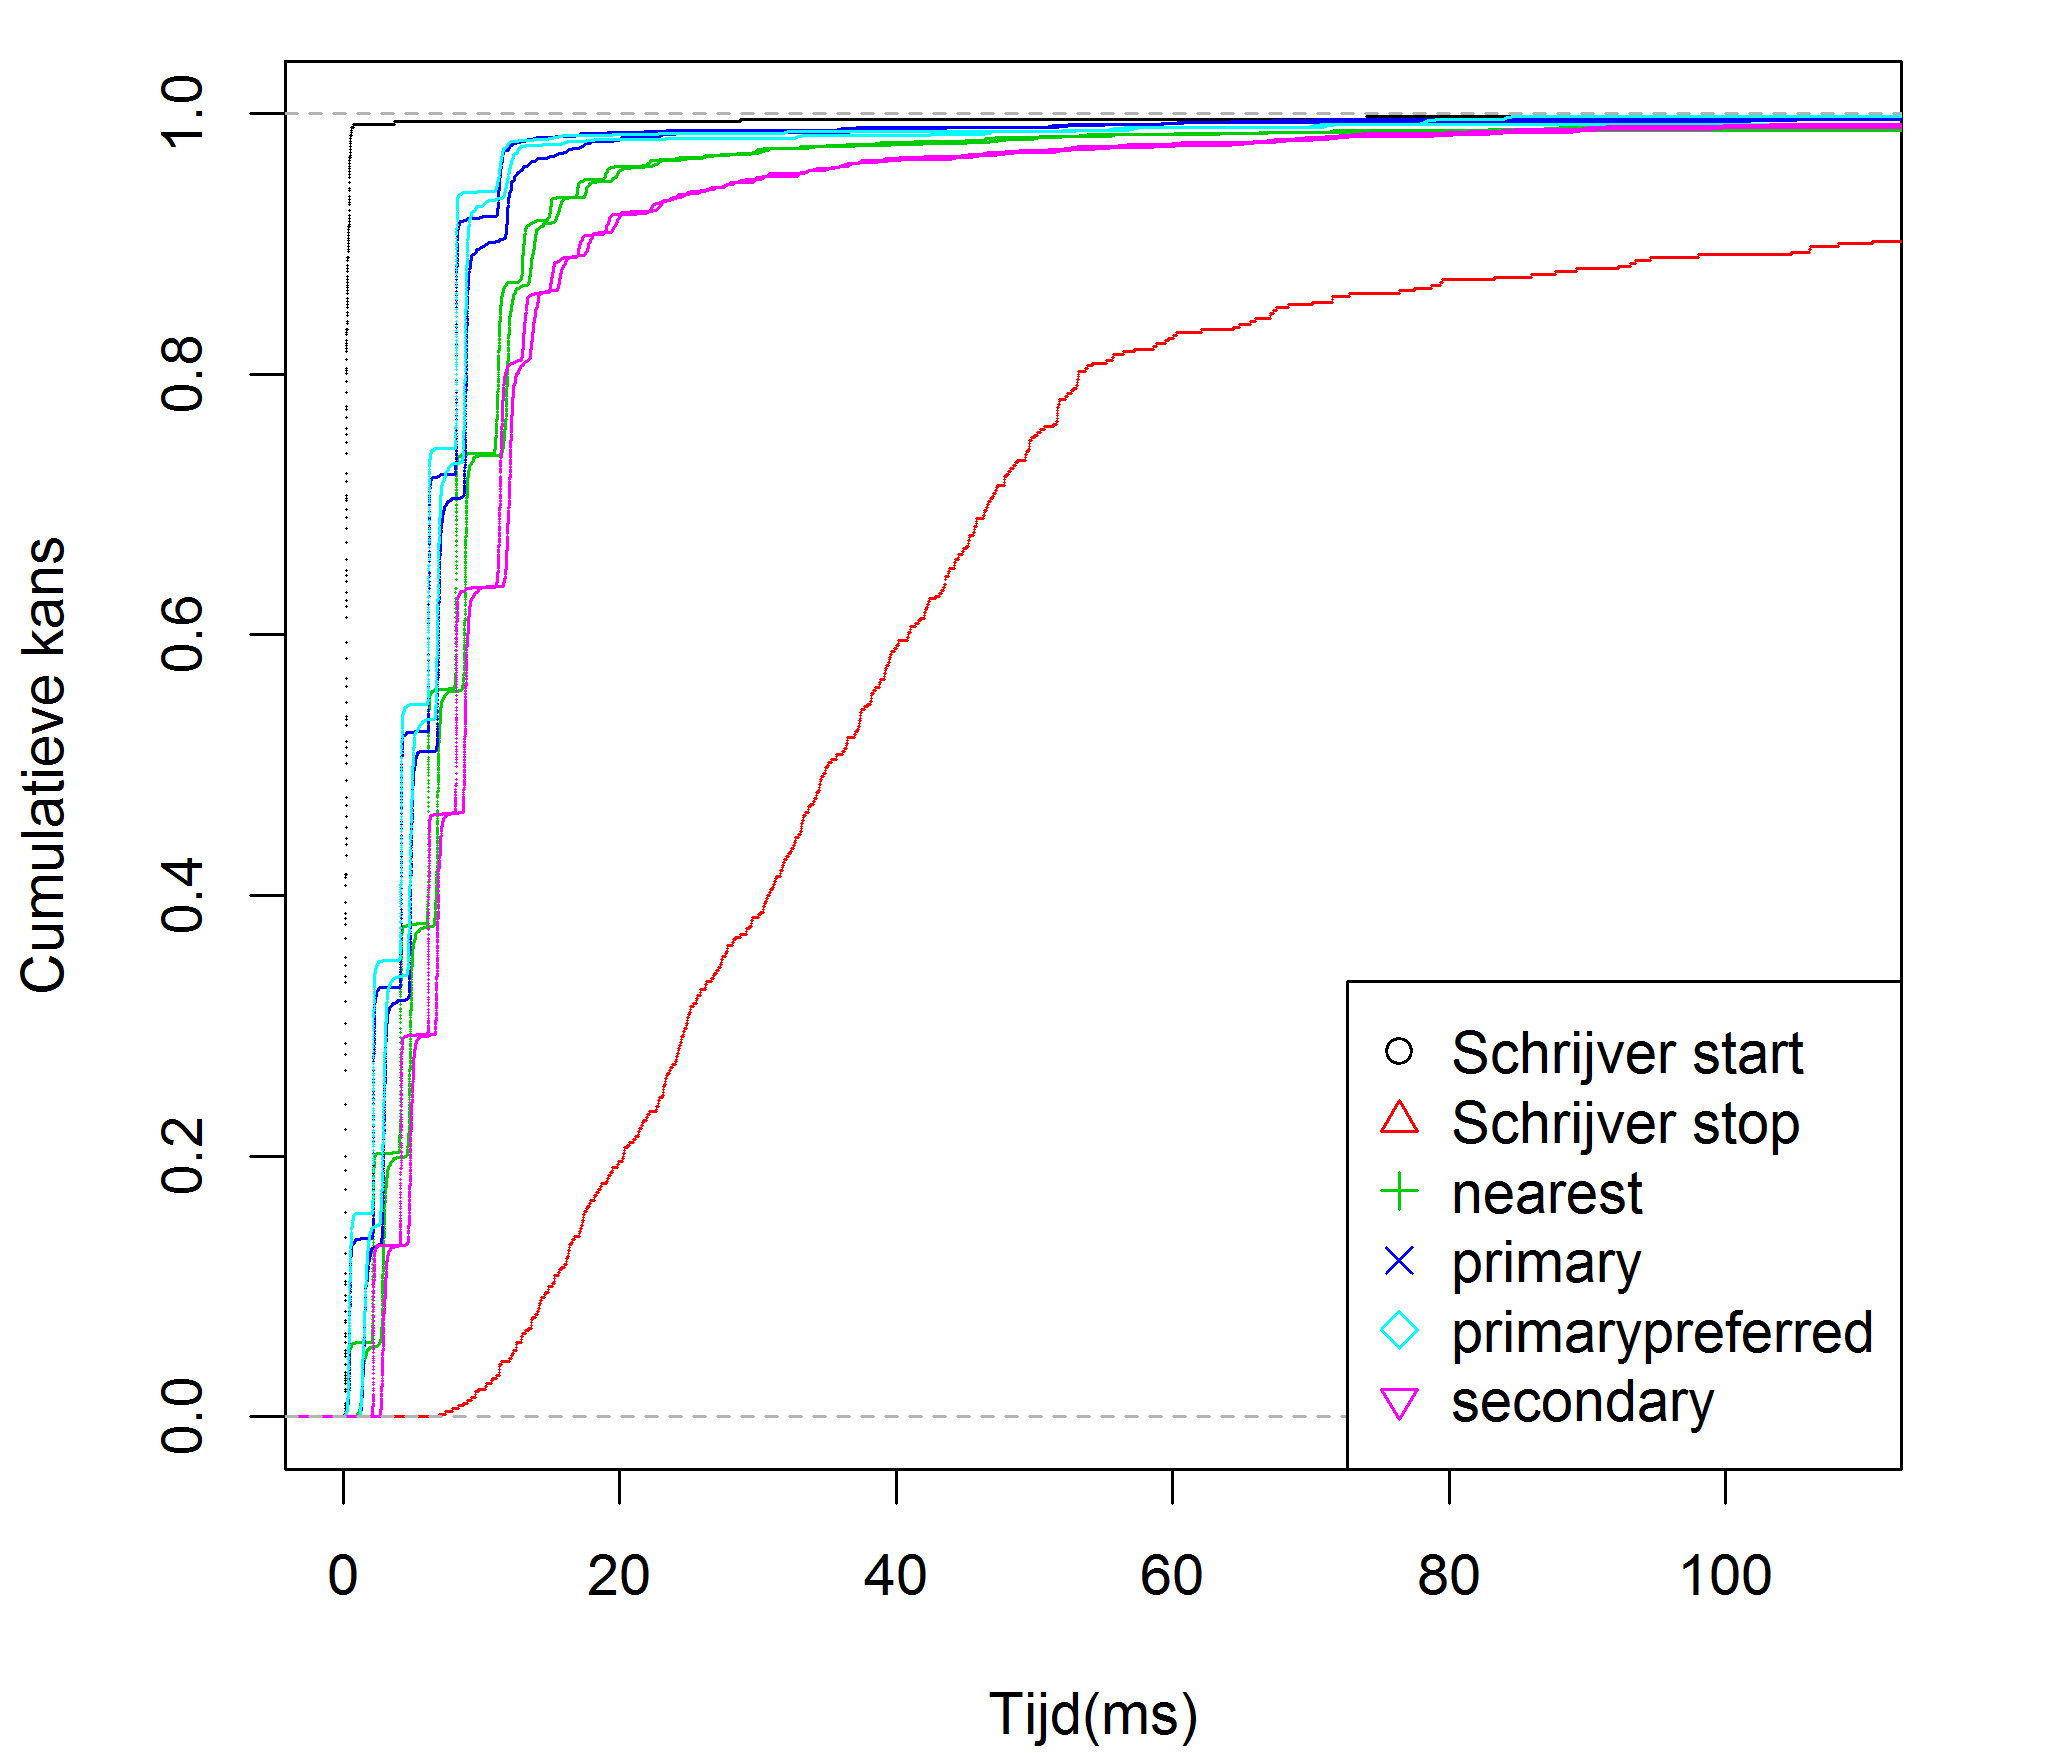
\includegraphics[width=.42\textwidth]{img/Observaties/MongoDB/ECDF-Reads-update-fsync_safe-all-2}}
%	\subfigure[Replica Safe Update]{\label{fig:consistentie-all-mongodb-replicasafe} 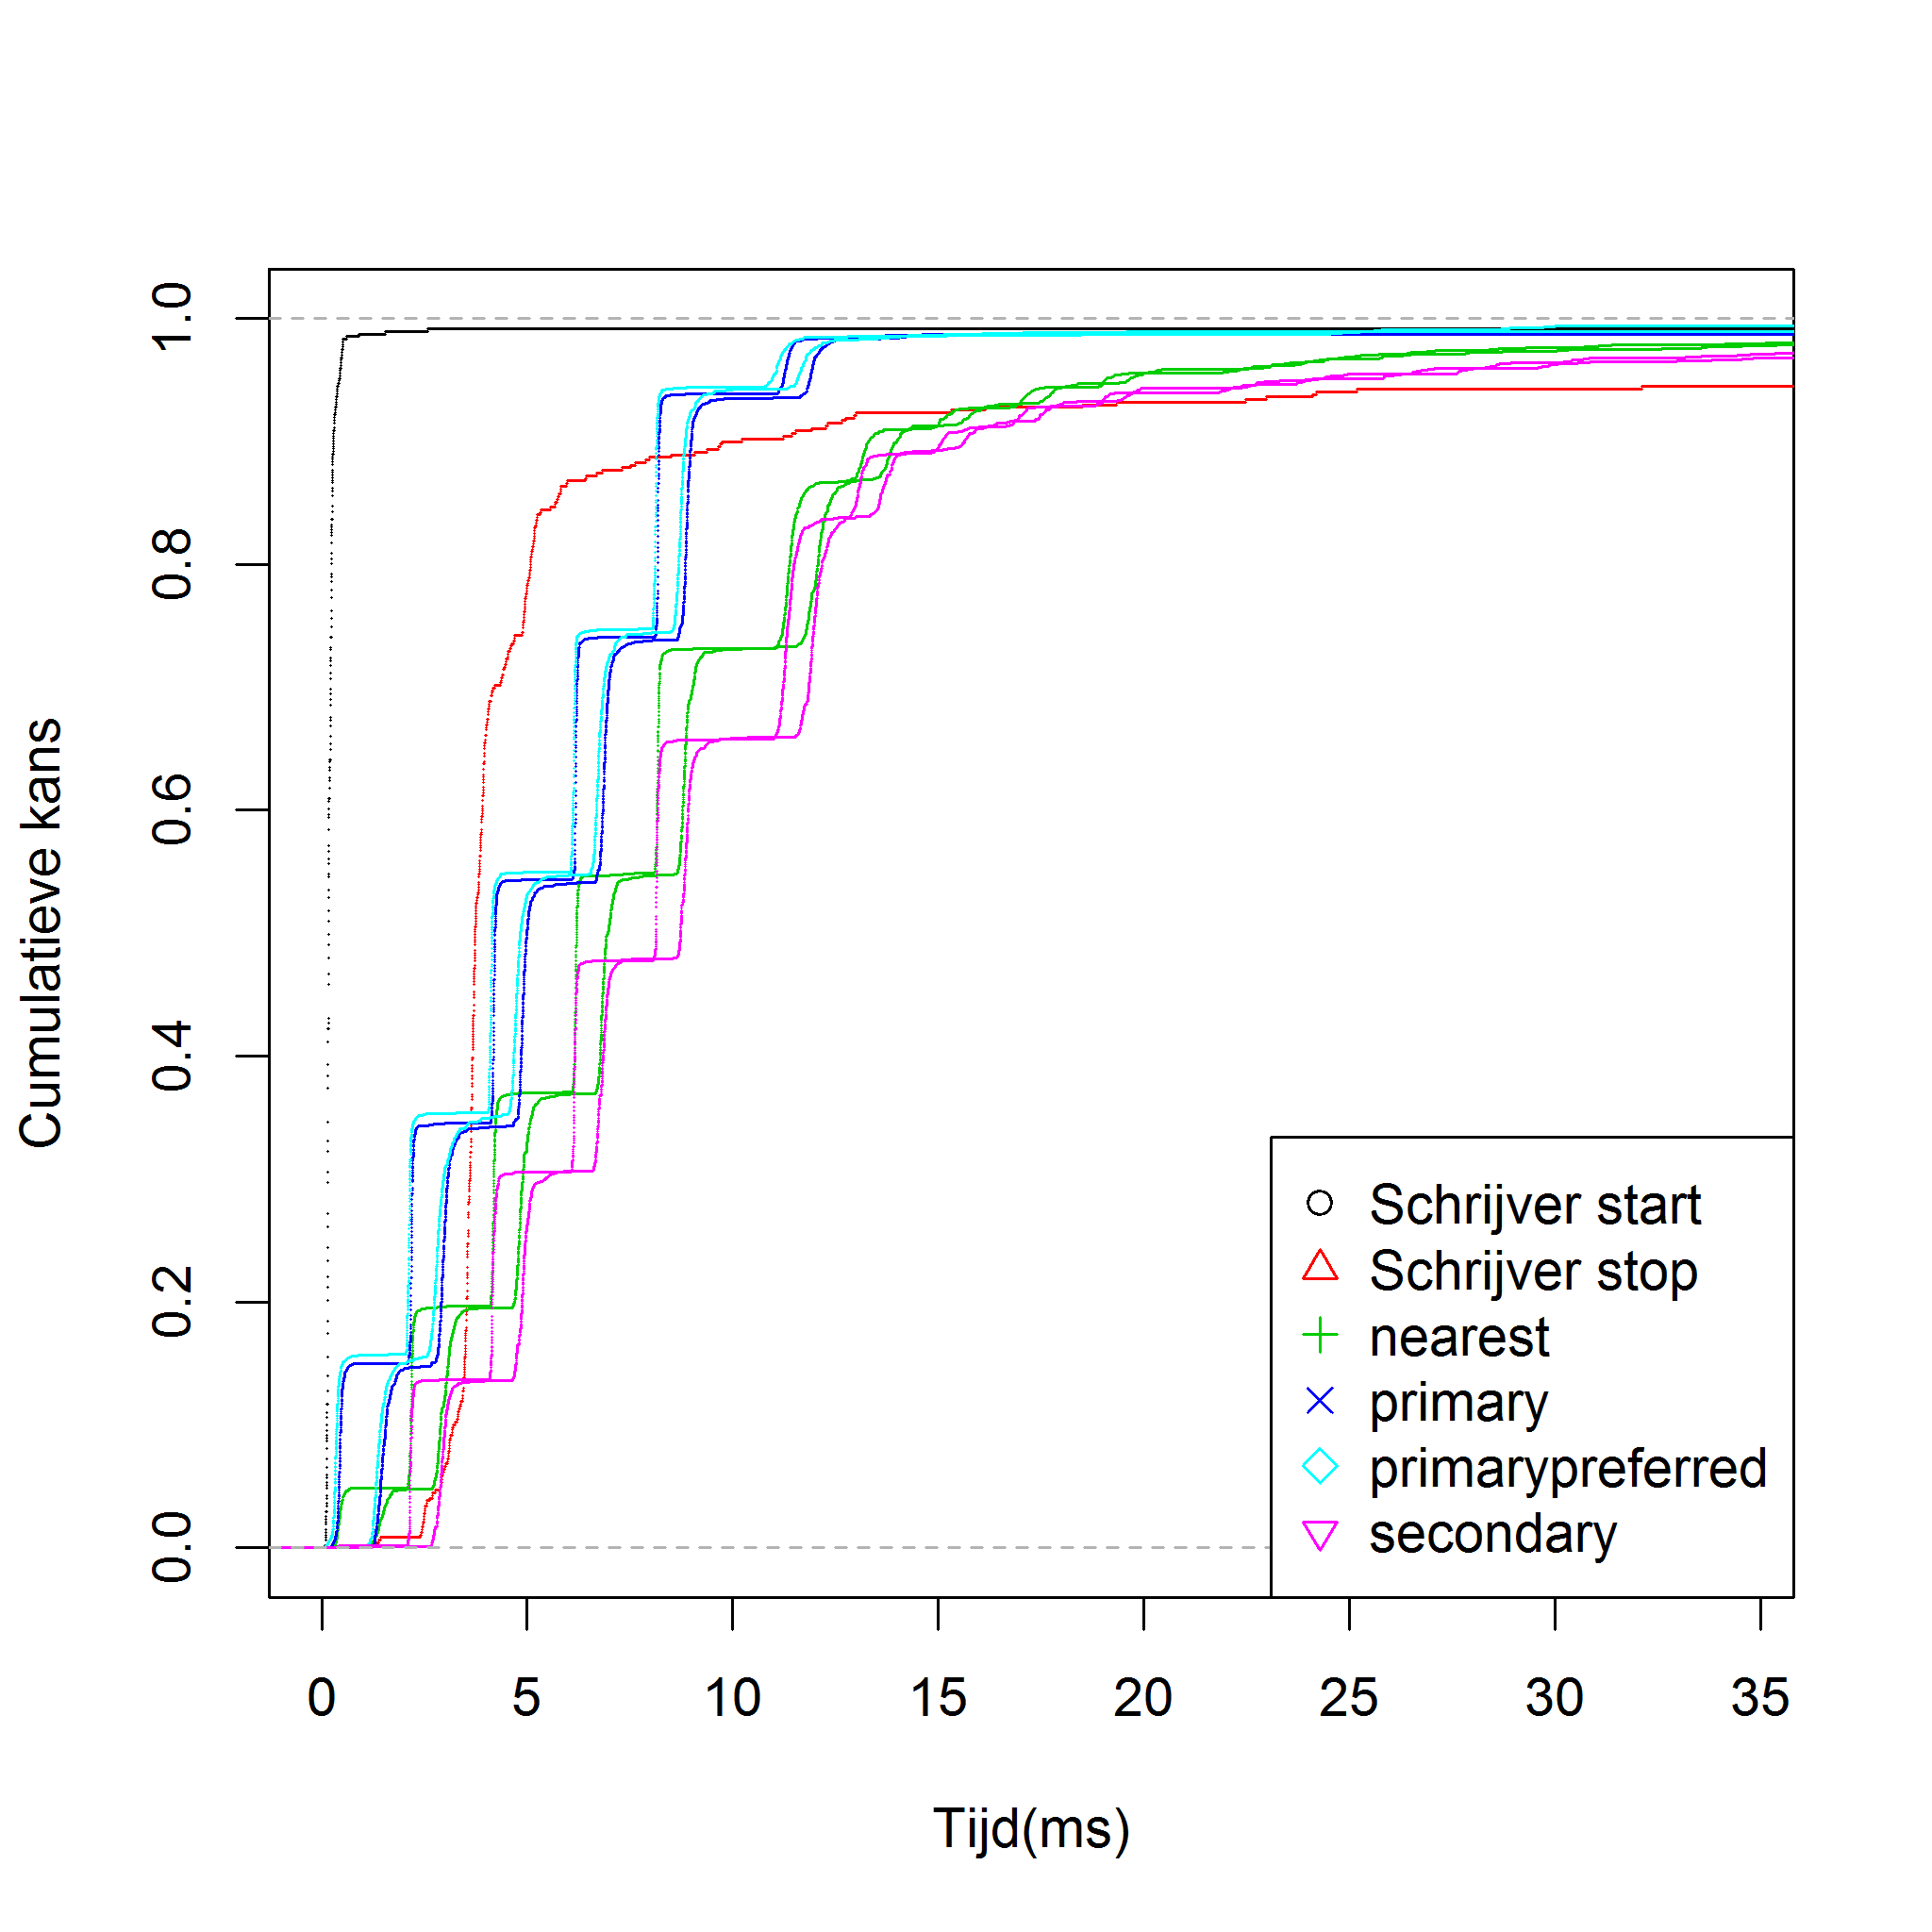
\includegraphics[width=.40\textwidth]{img/Observaties/MongoDB/ECDF-Reads-update-replicas_safe-all-2}}
%	\subfigure[Majority Update]{\label{fig:consistentie-mongodb-all-majority} 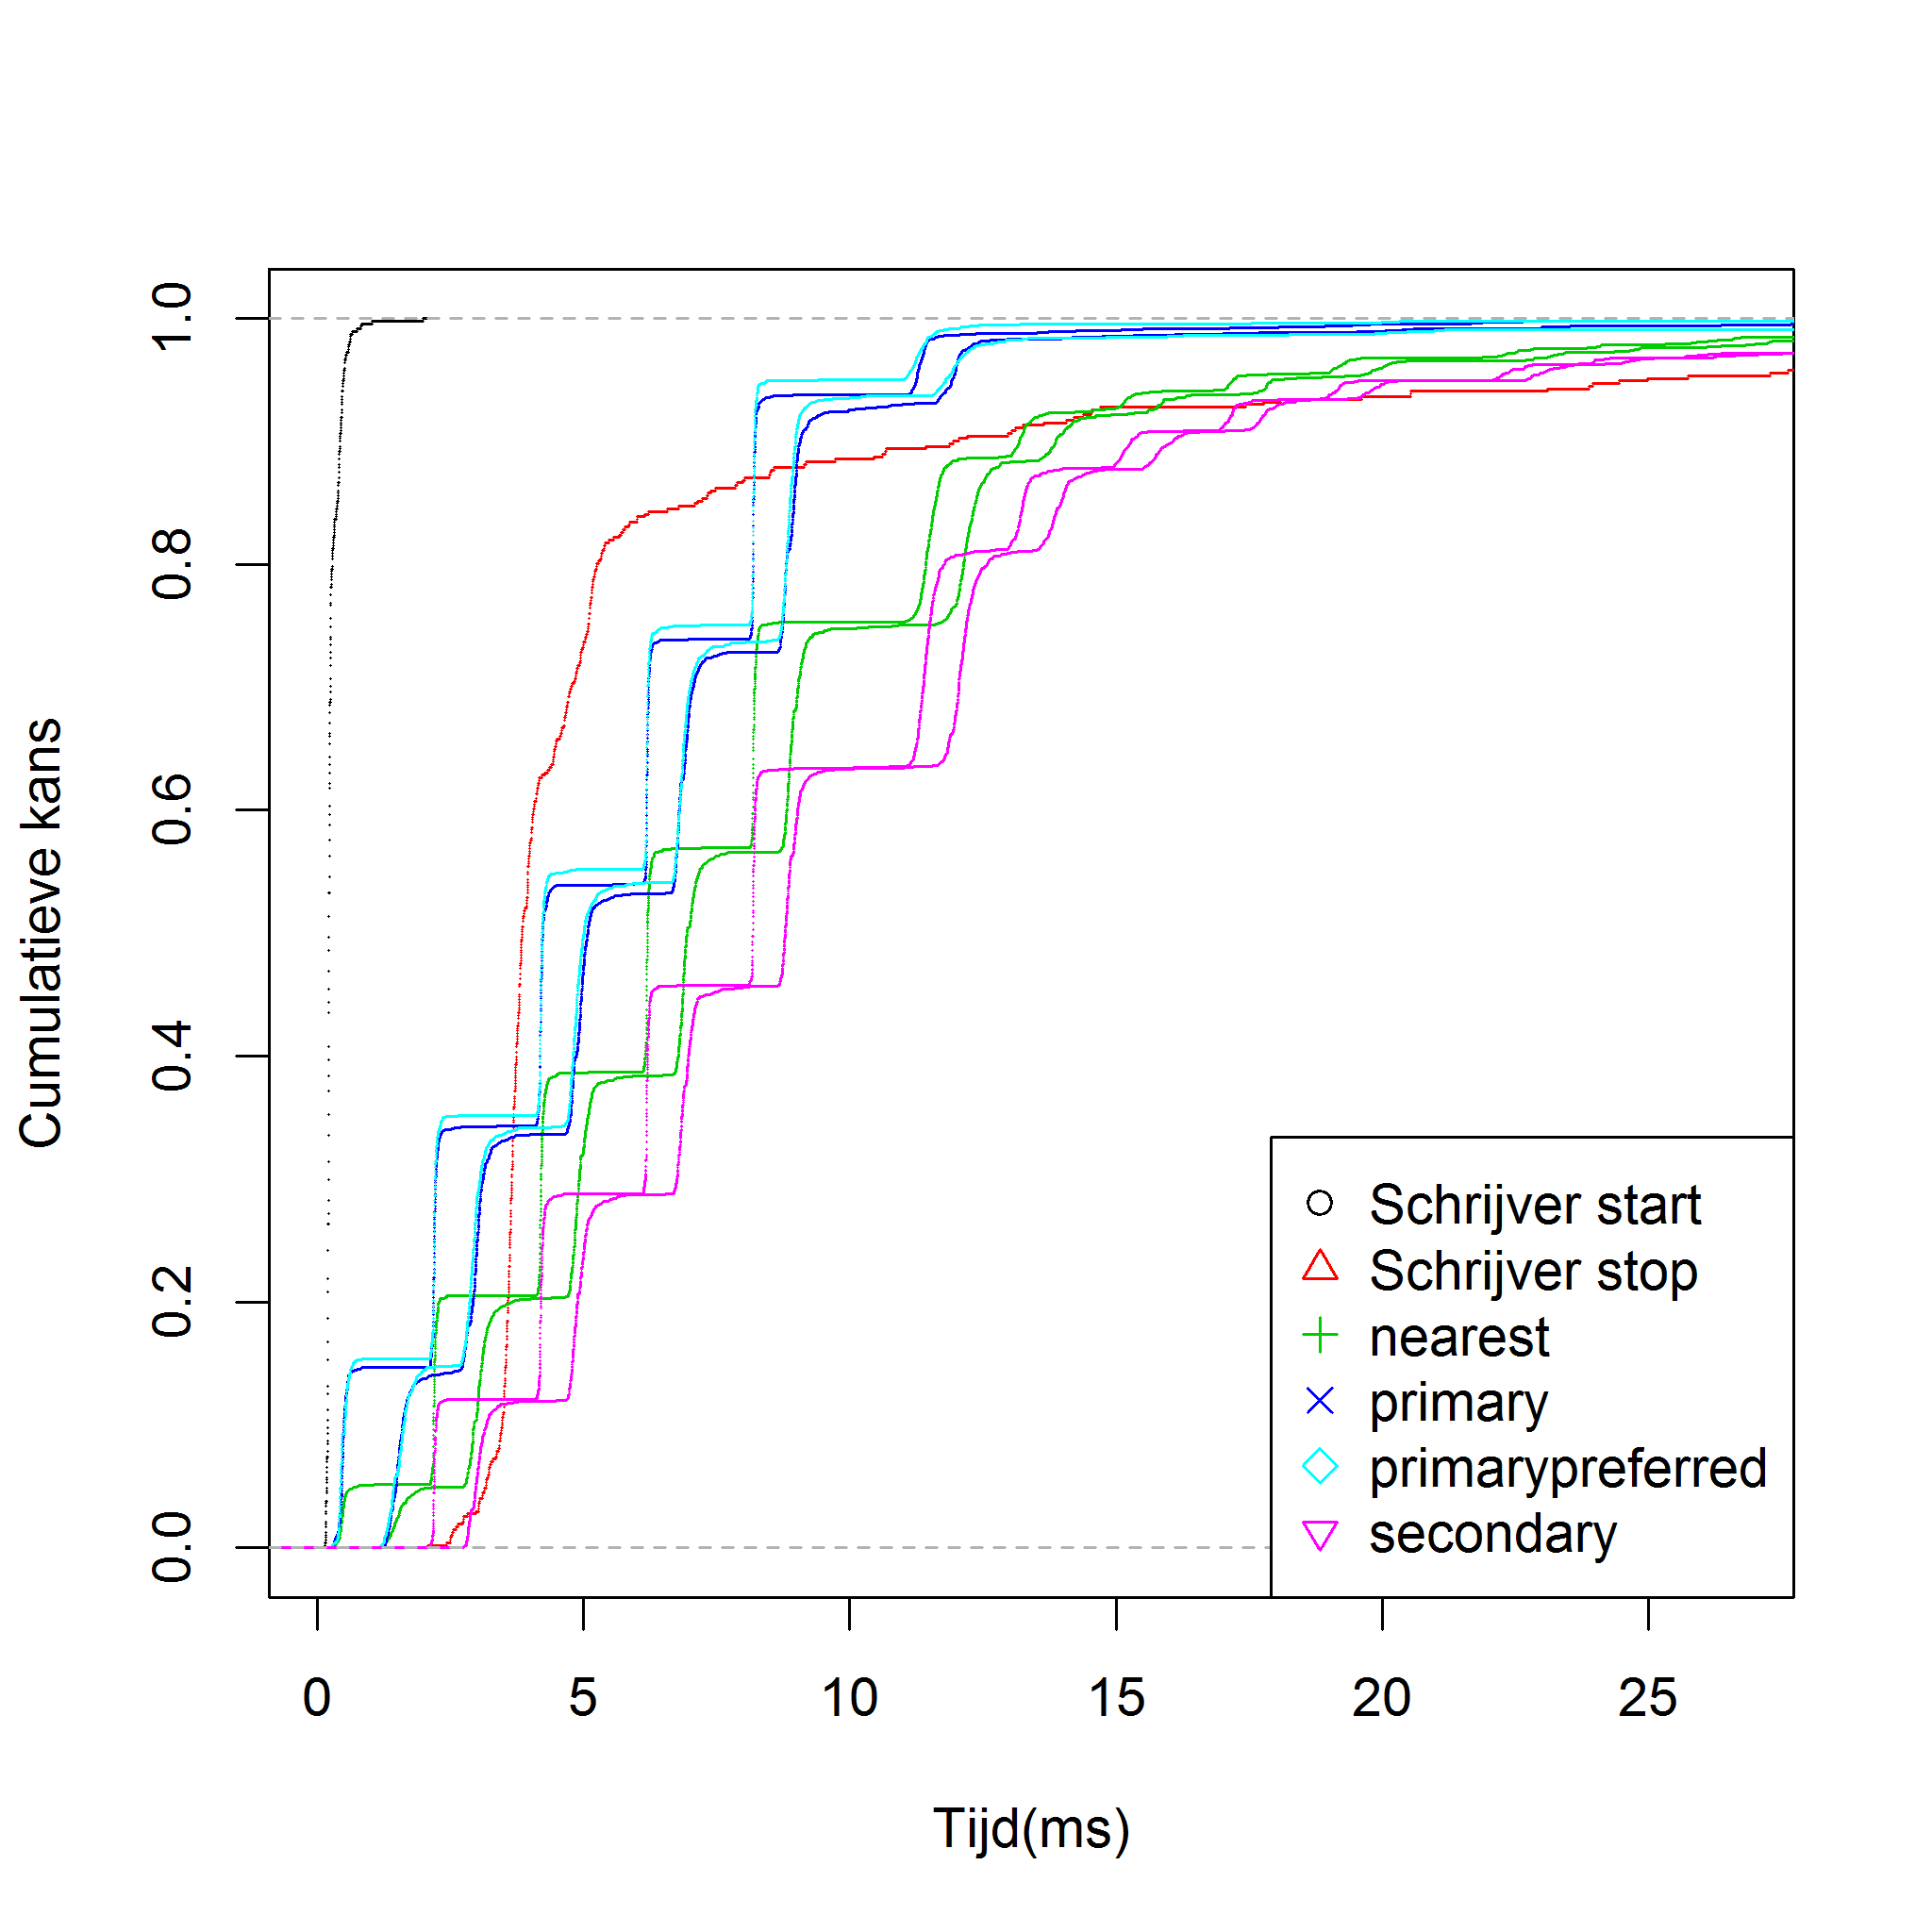
\includegraphics[width=.40\textwidth]{img/Observaties/MongoDB/ECDF-Reads-update-majority-all-2}}
%	\subfigure[Majority Insert]{\label{fig:consistentie-mongodb-all-majority-insert} 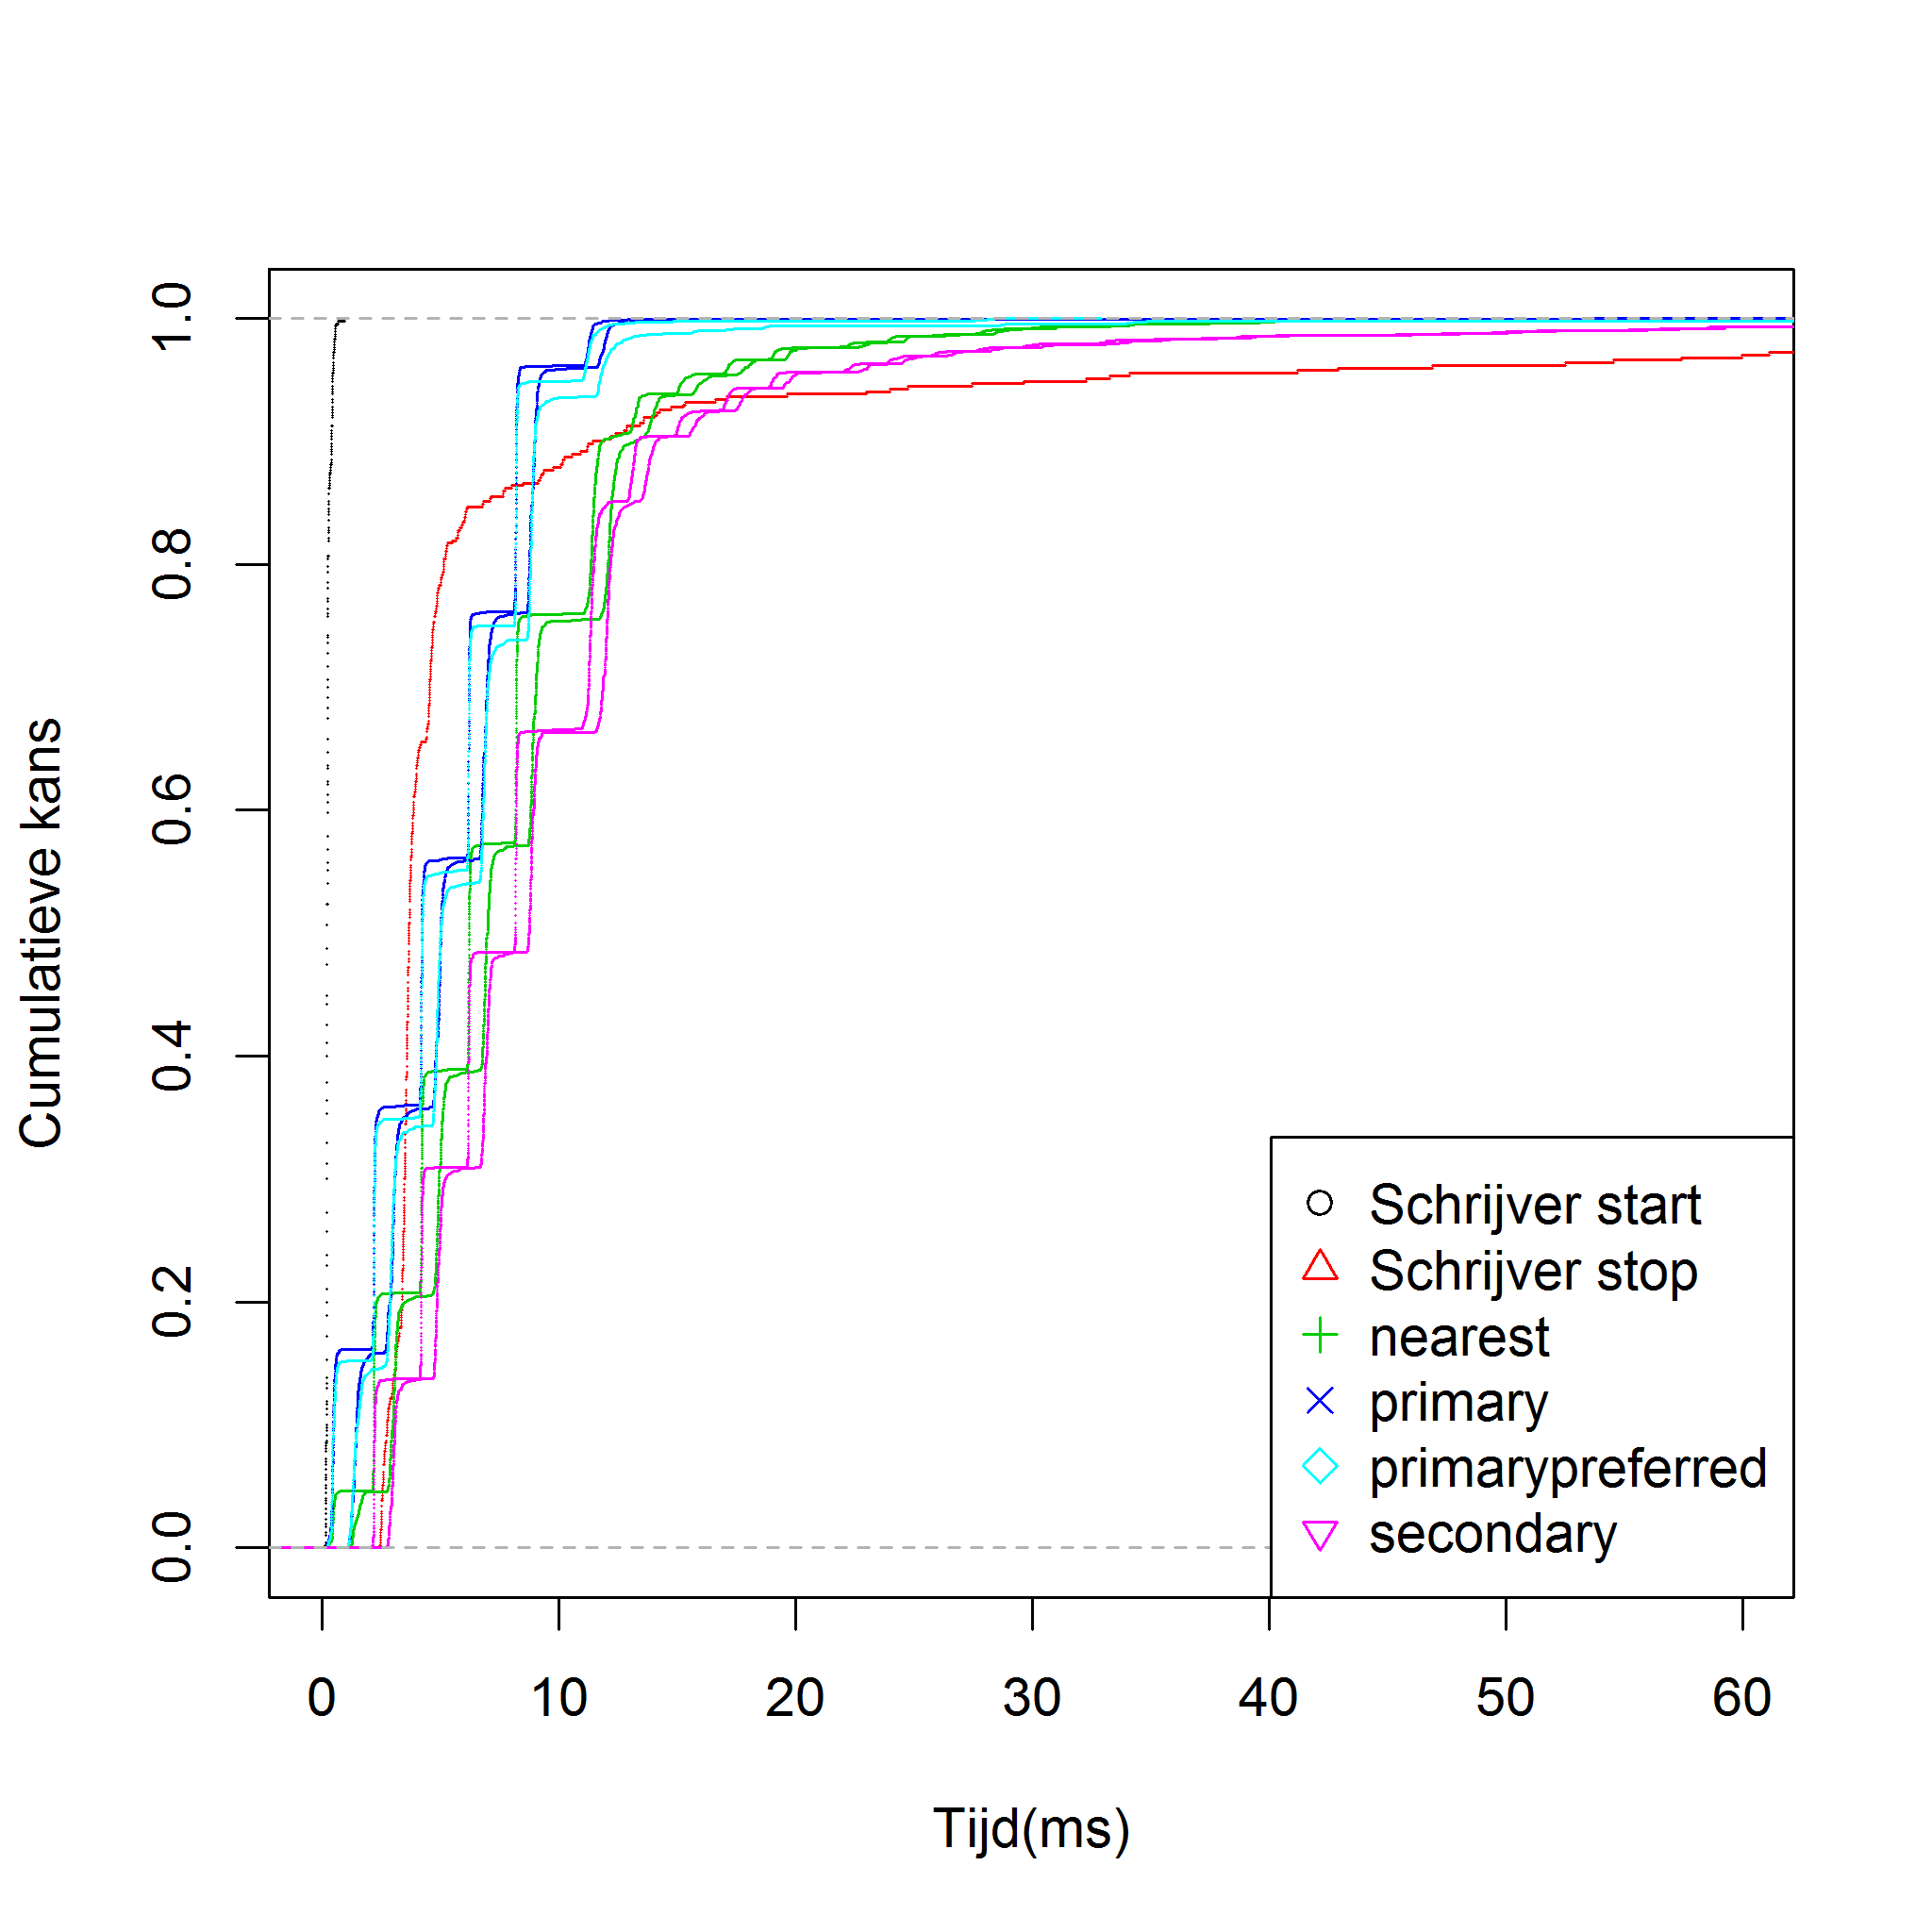
\includegraphics[width=.40\textwidth]{img/Observaties/MongoDB/ECDF-Reads-insert-majority-all-2}}
%	\caption{Consistentie: Overzicht van MongoDB op de consistentie testen voor alle lezers gecombineerd met een 97-percentiel (voor de lezers) met start en stoptijden in dezelfde kleur. }
%	\label{fig:consistentie-mongodb-all}
%\end{figure}

%\begin{figure}[ht!] 
%	\centering
%	\subfigure[Normal Update]{\label{fig:consistentie-mongodb-R2-normal} 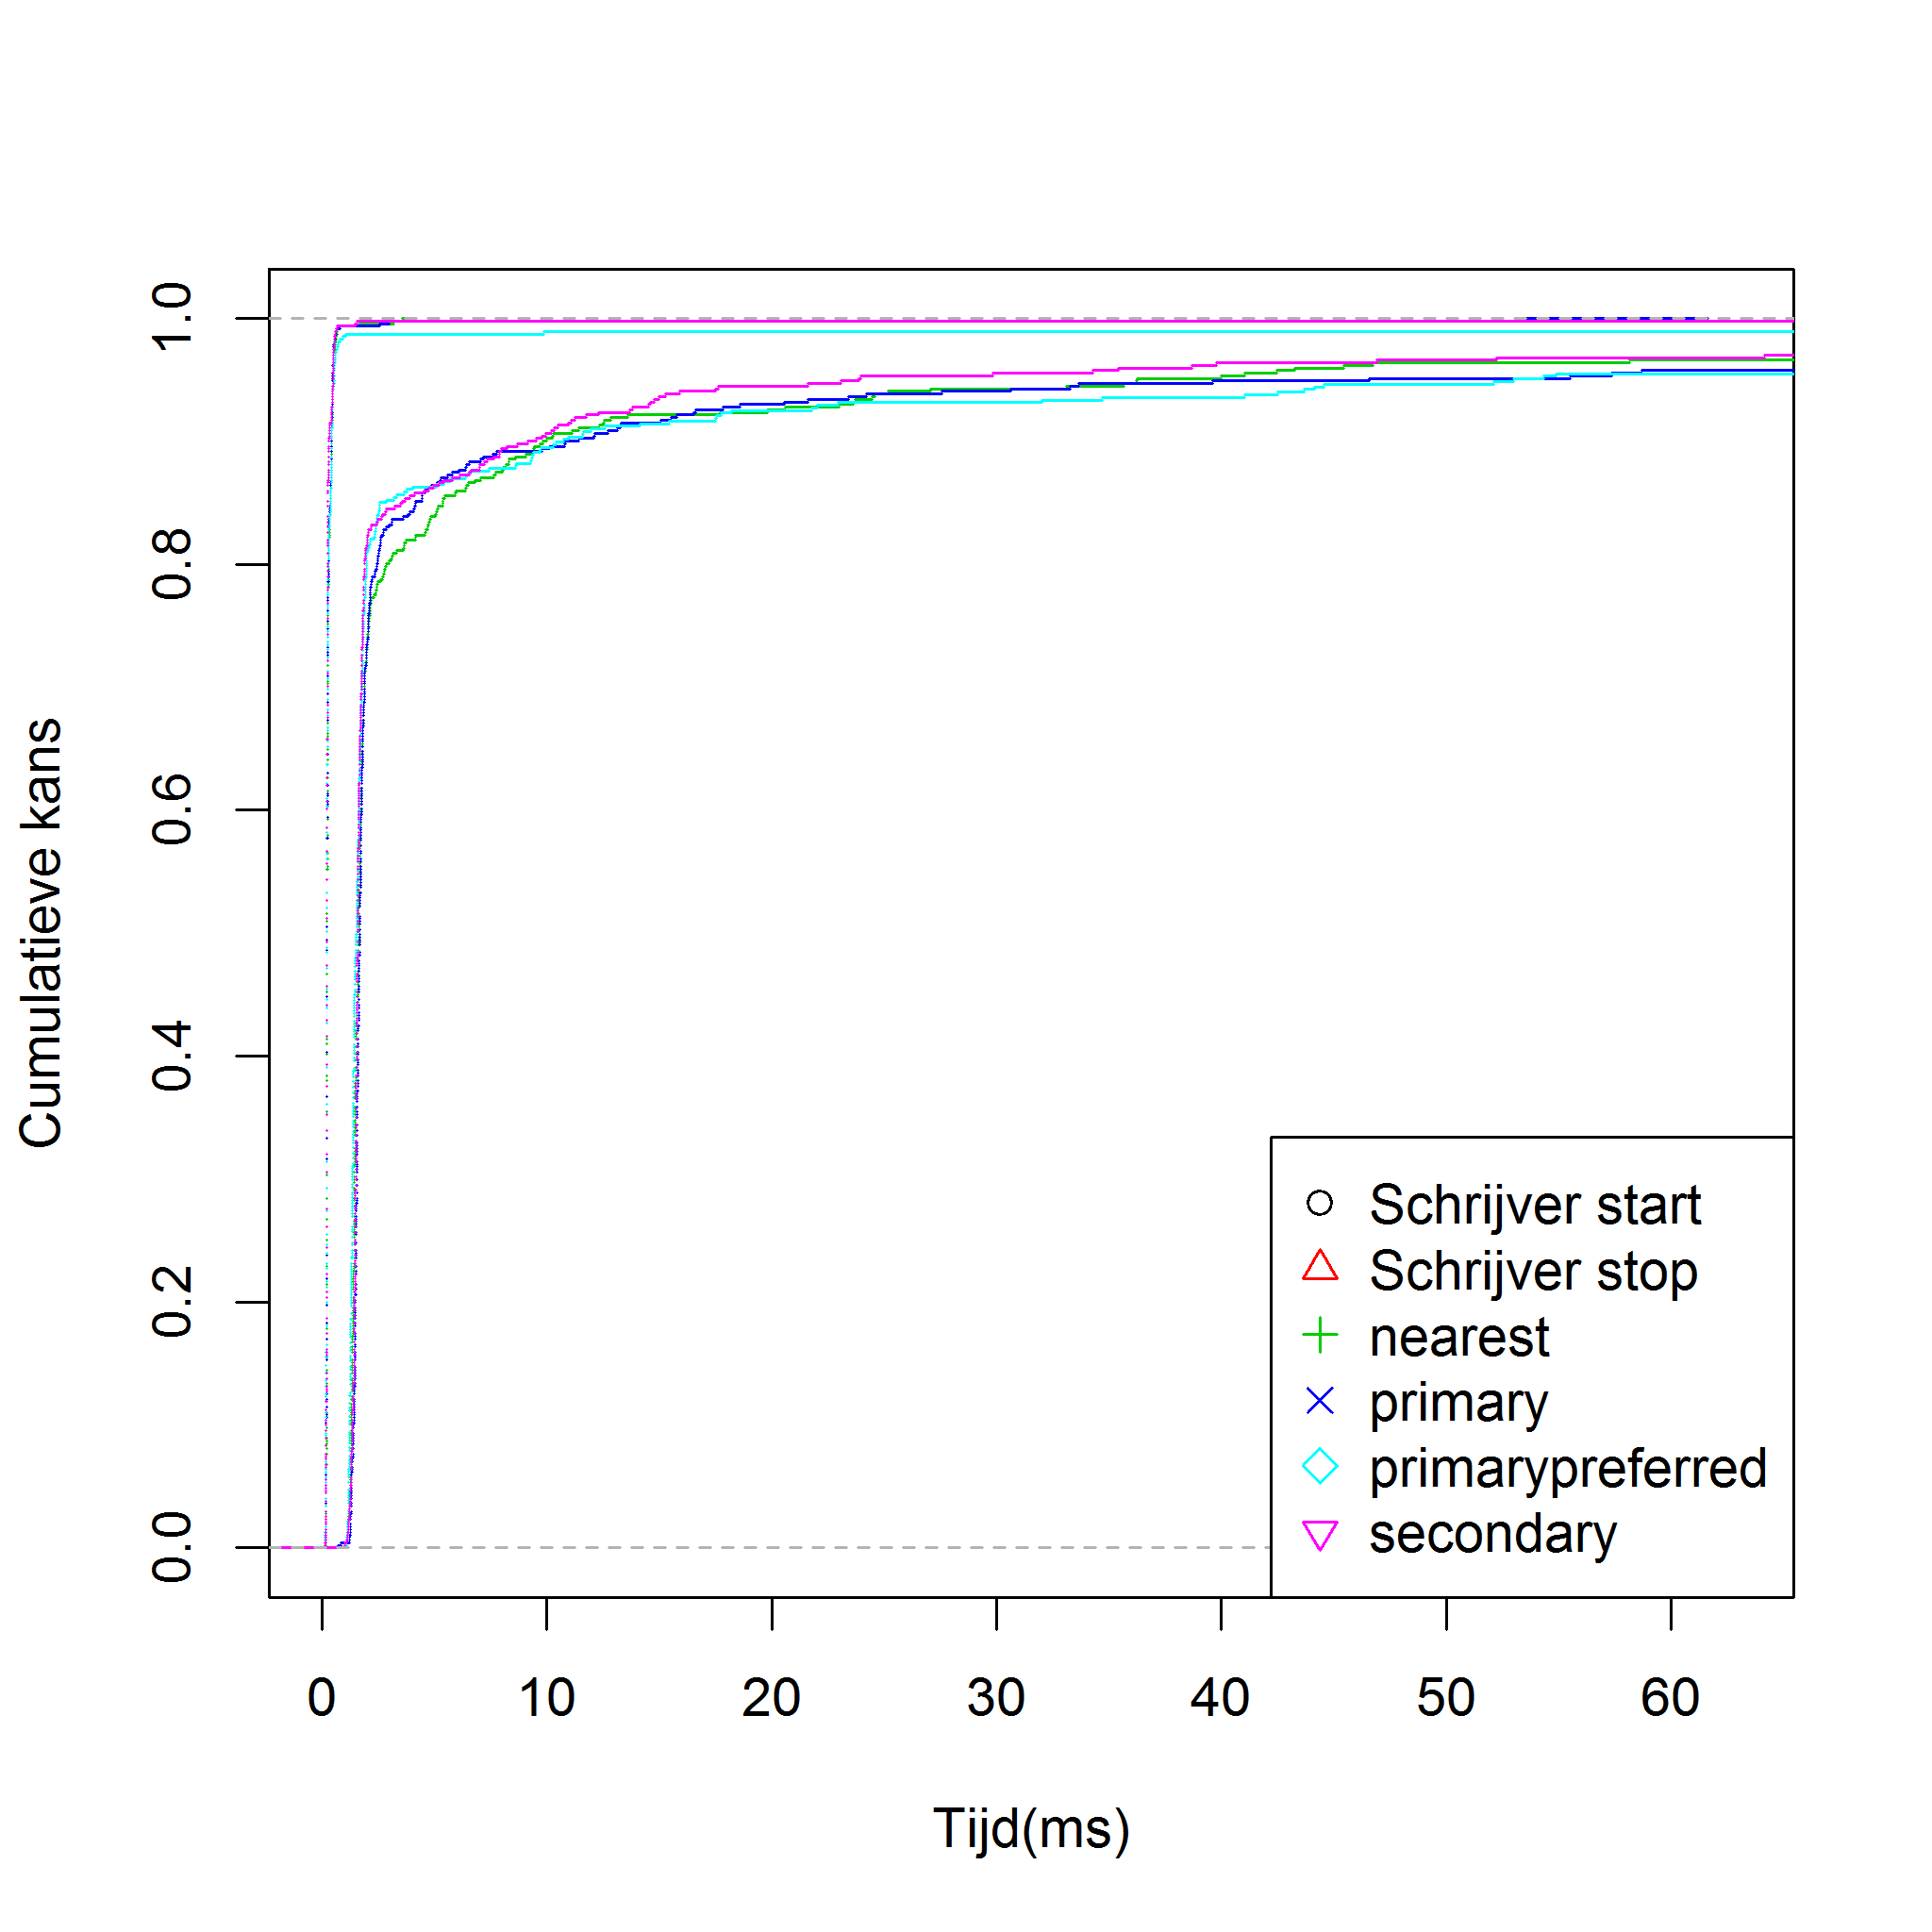
\includegraphics[width=.40\textwidth]{img/Observaties/MongoDB/ECDF-Reads-update-normal-1-2}}
%	\subfigure[Safe Update]{\label{fig:consistentie-mongodb-R2-safe} 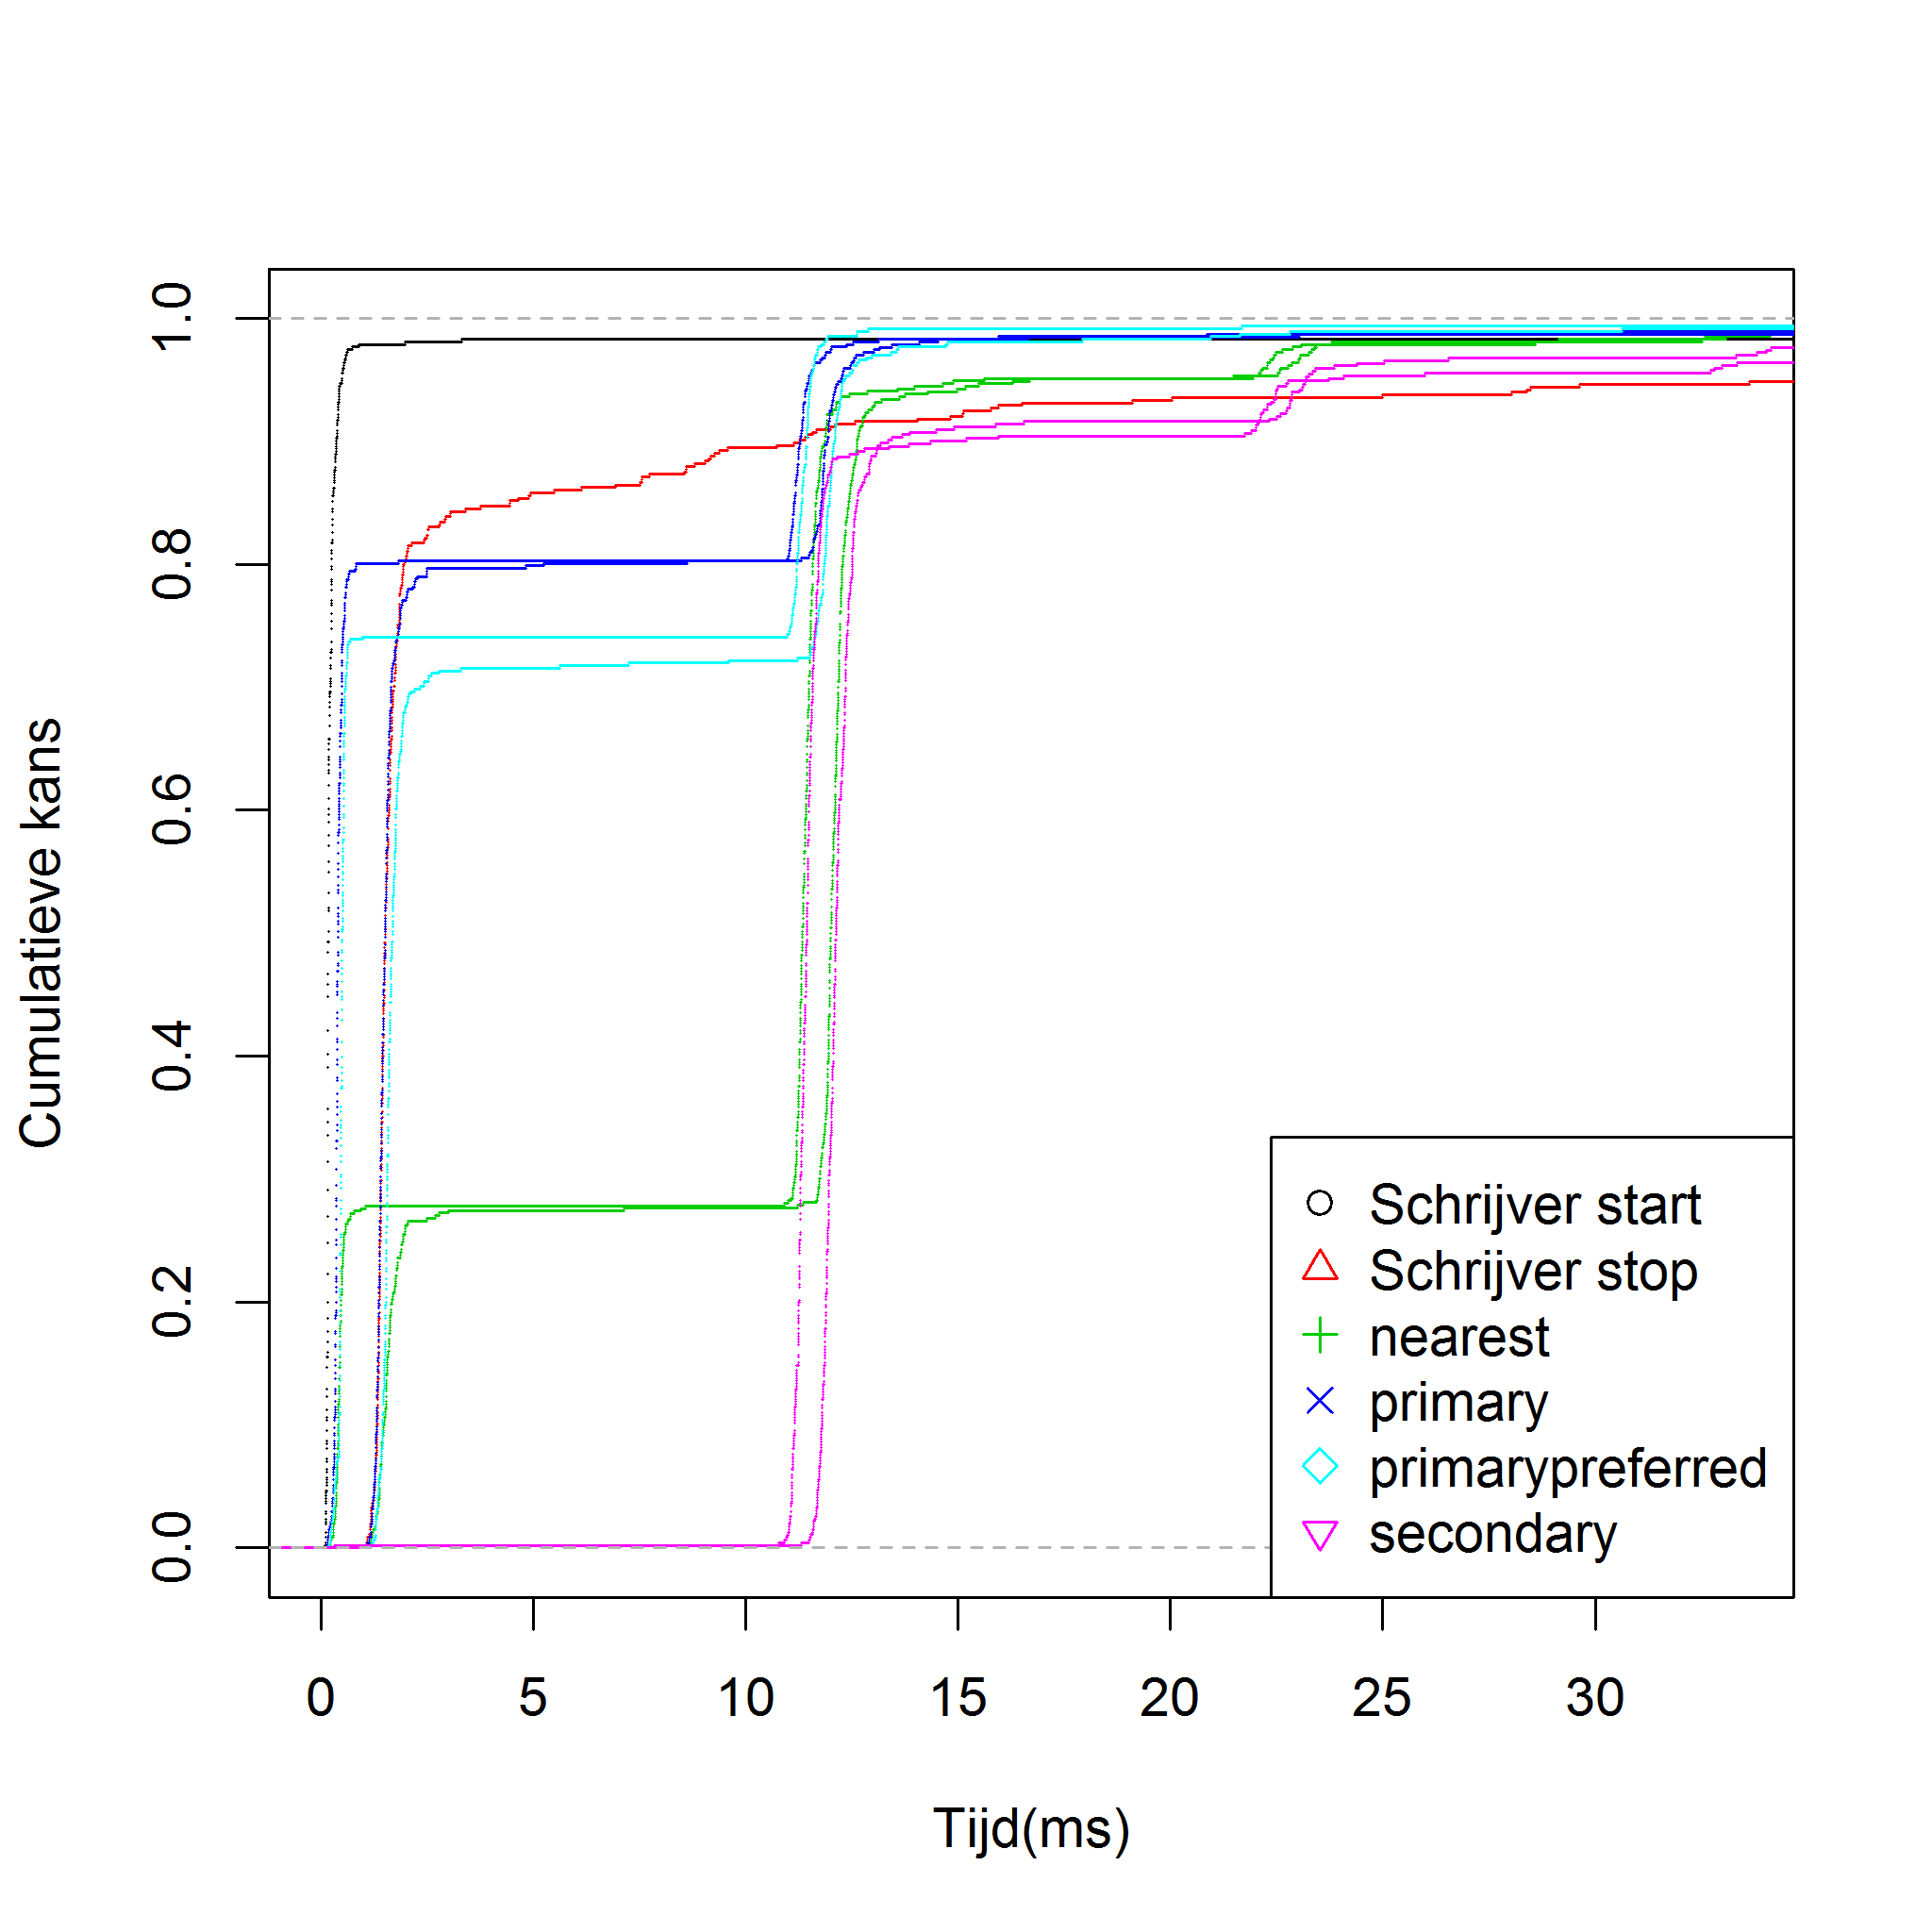
\includegraphics[width=.40\textwidth]{img/Observaties/MongoDB/ECDF-Reads-update-safe-1-2}}
%	\subfigure[Fsync Safe Update]{\label{fig:consistentie-mongodb-R2-fsync} 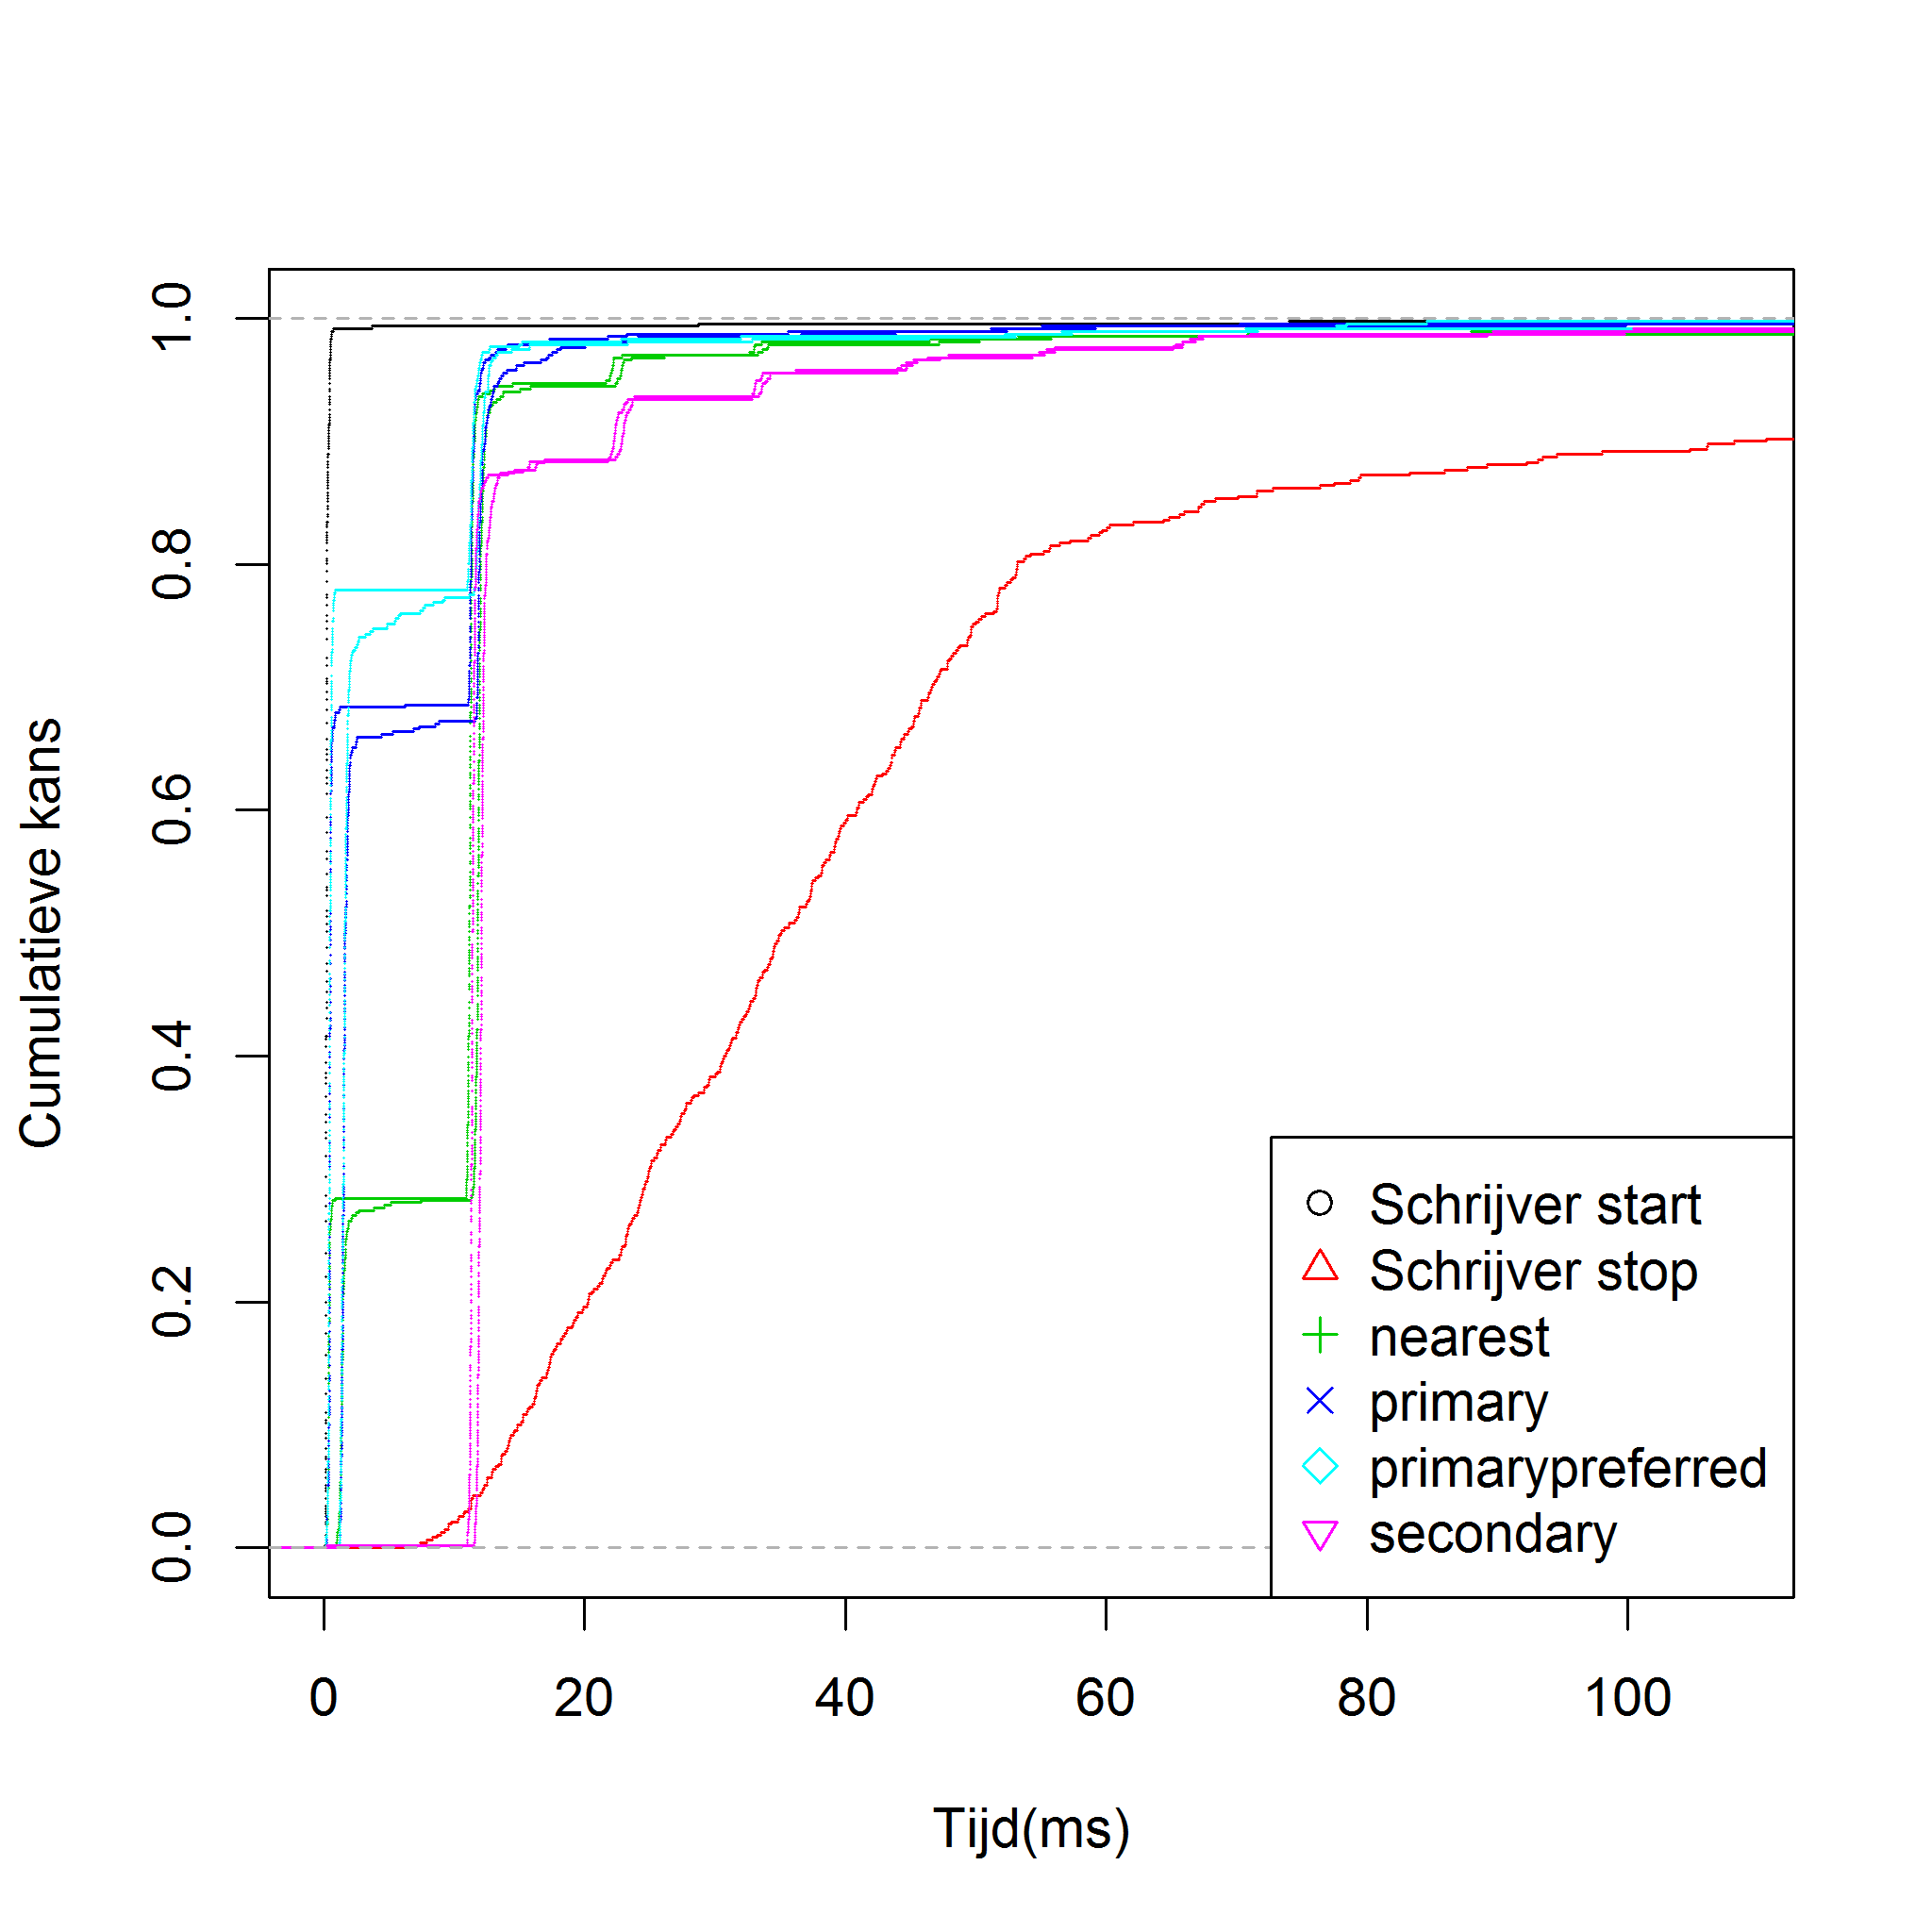
\includegraphics[width=.40\textwidth]{img/Observaties/MongoDB/ECDF-Reads-update-fsync_safe-1-2}}
%	\subfigure[Replica Safe Update]{\label{fig:consistentie-mongodb-R2-replicasafe} 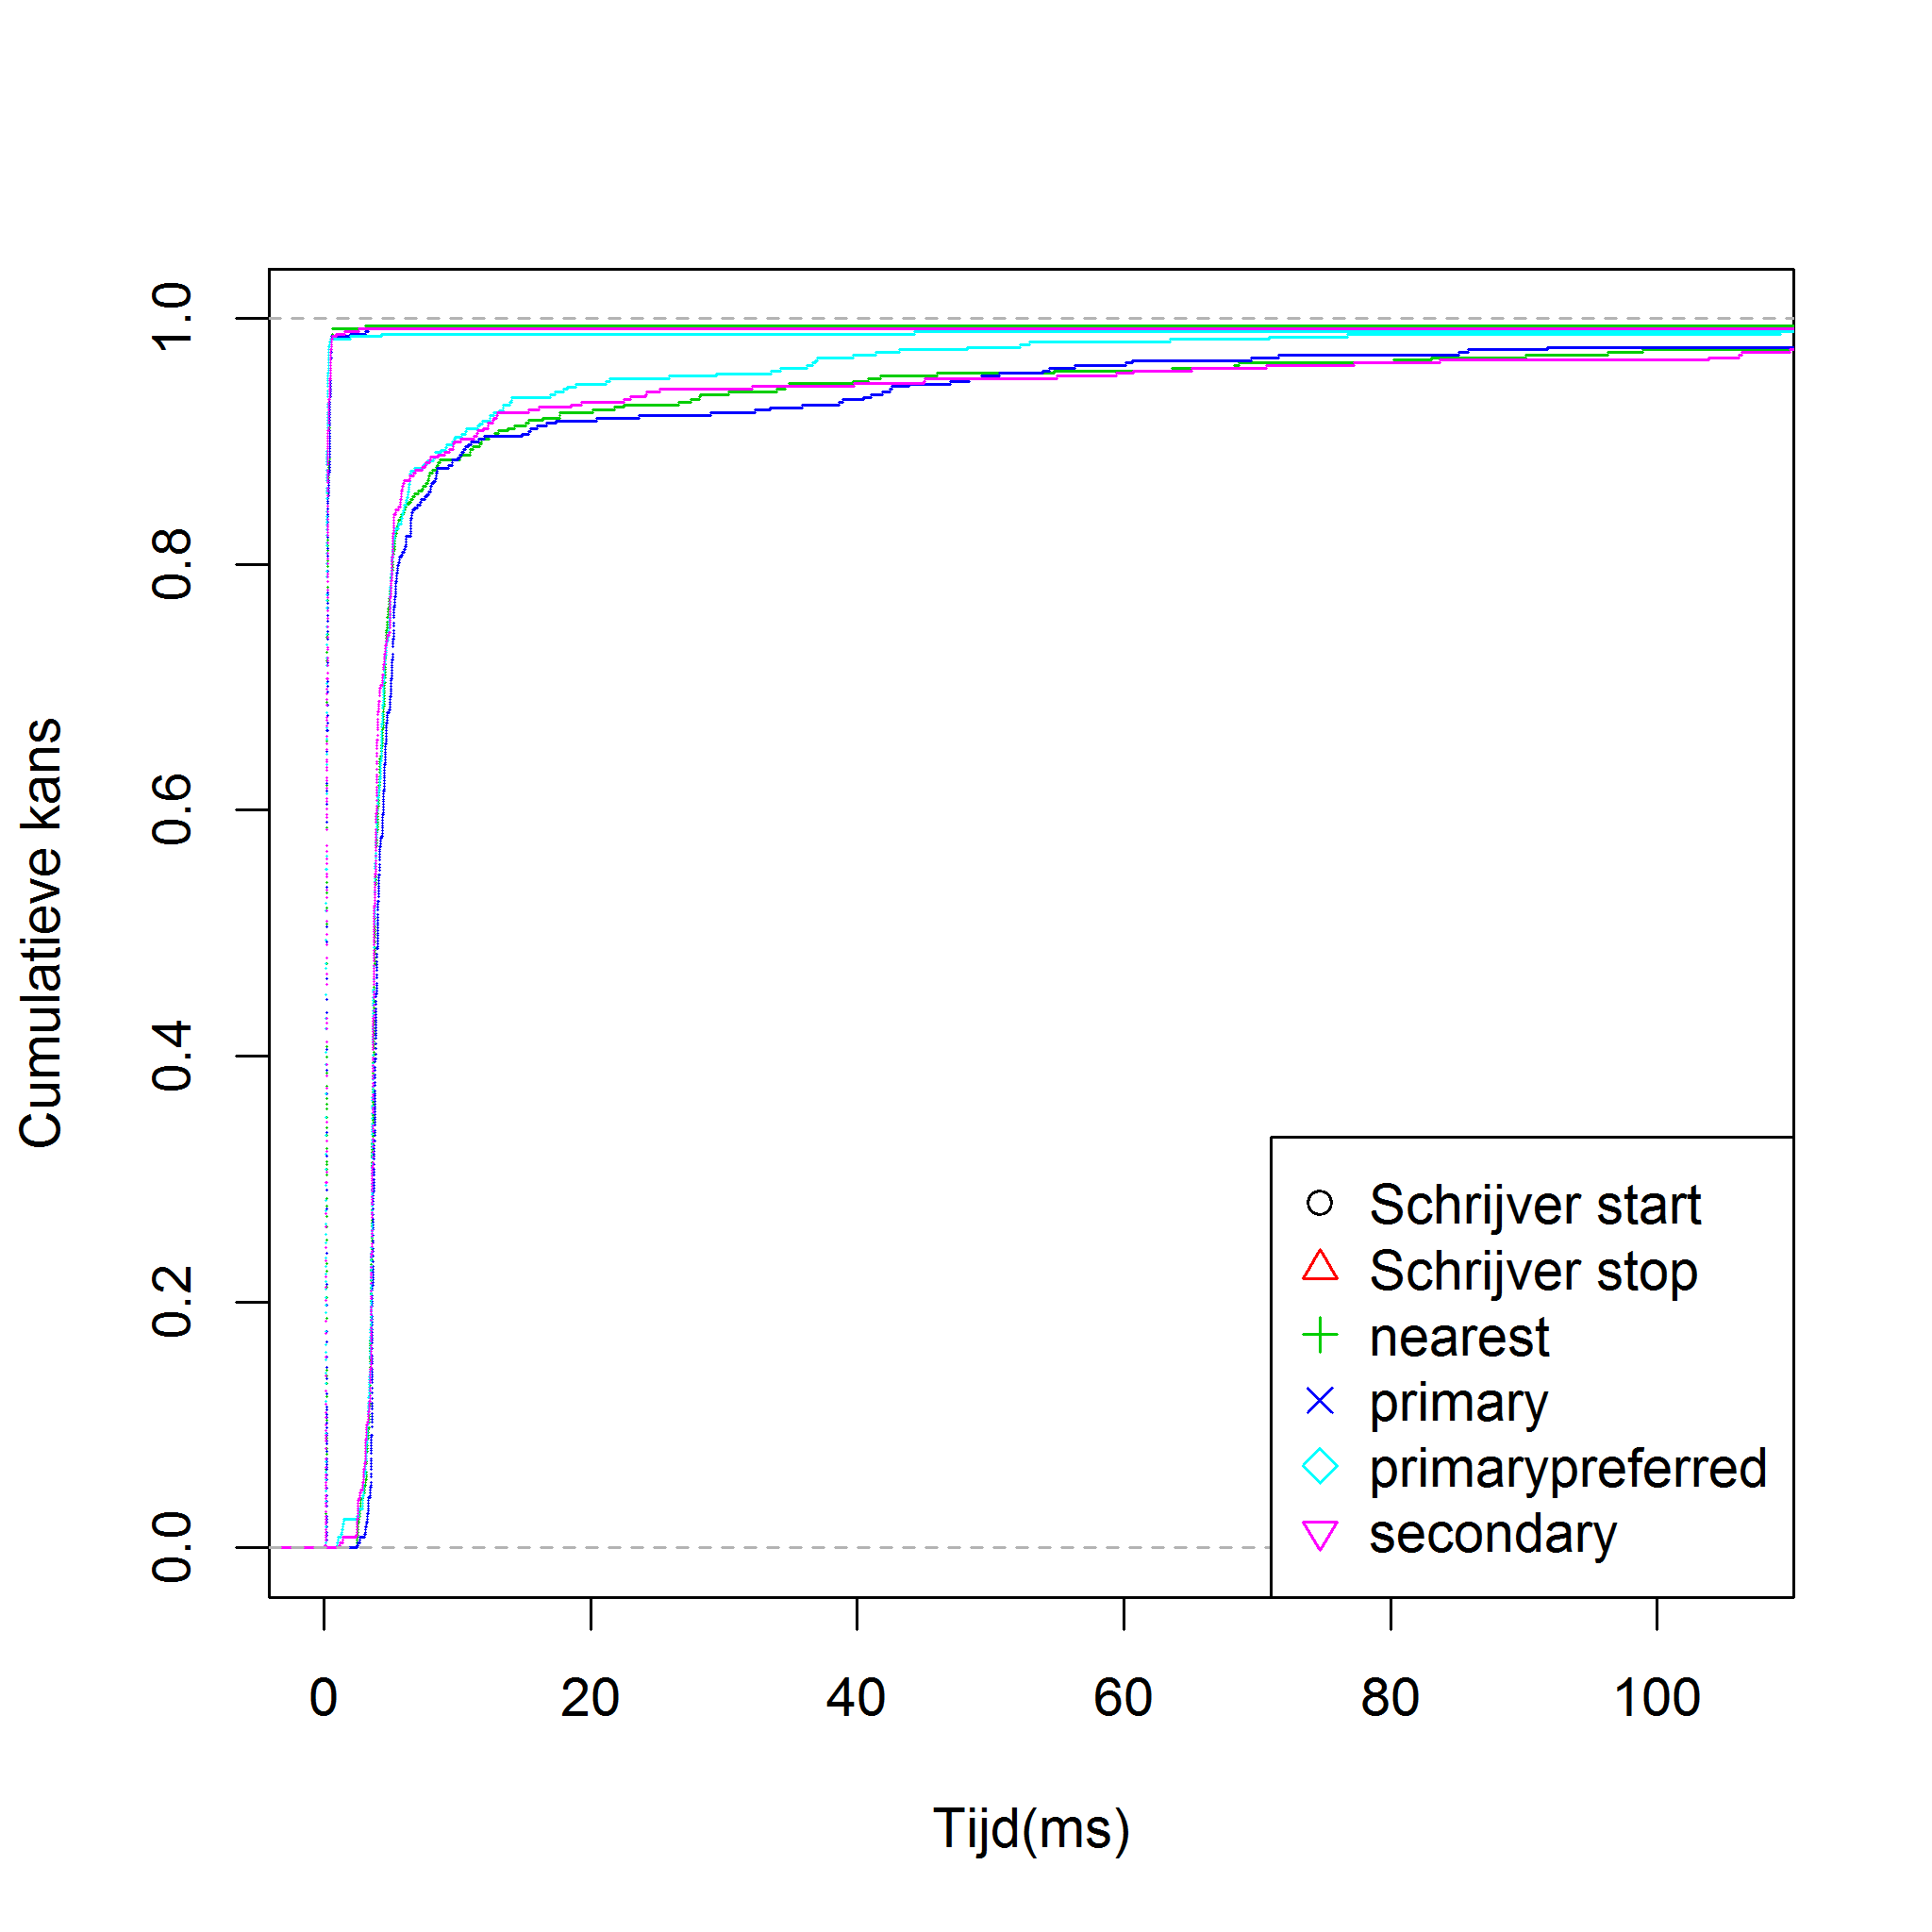
\includegraphics[width=.40\textwidth]{img/Observaties/MongoDB/ECDF-Reads-update-replicas_safe-1-2}}
%	\subfigure[Majority Update]{\label{fig:consistentie-mongodb-R2-majority} 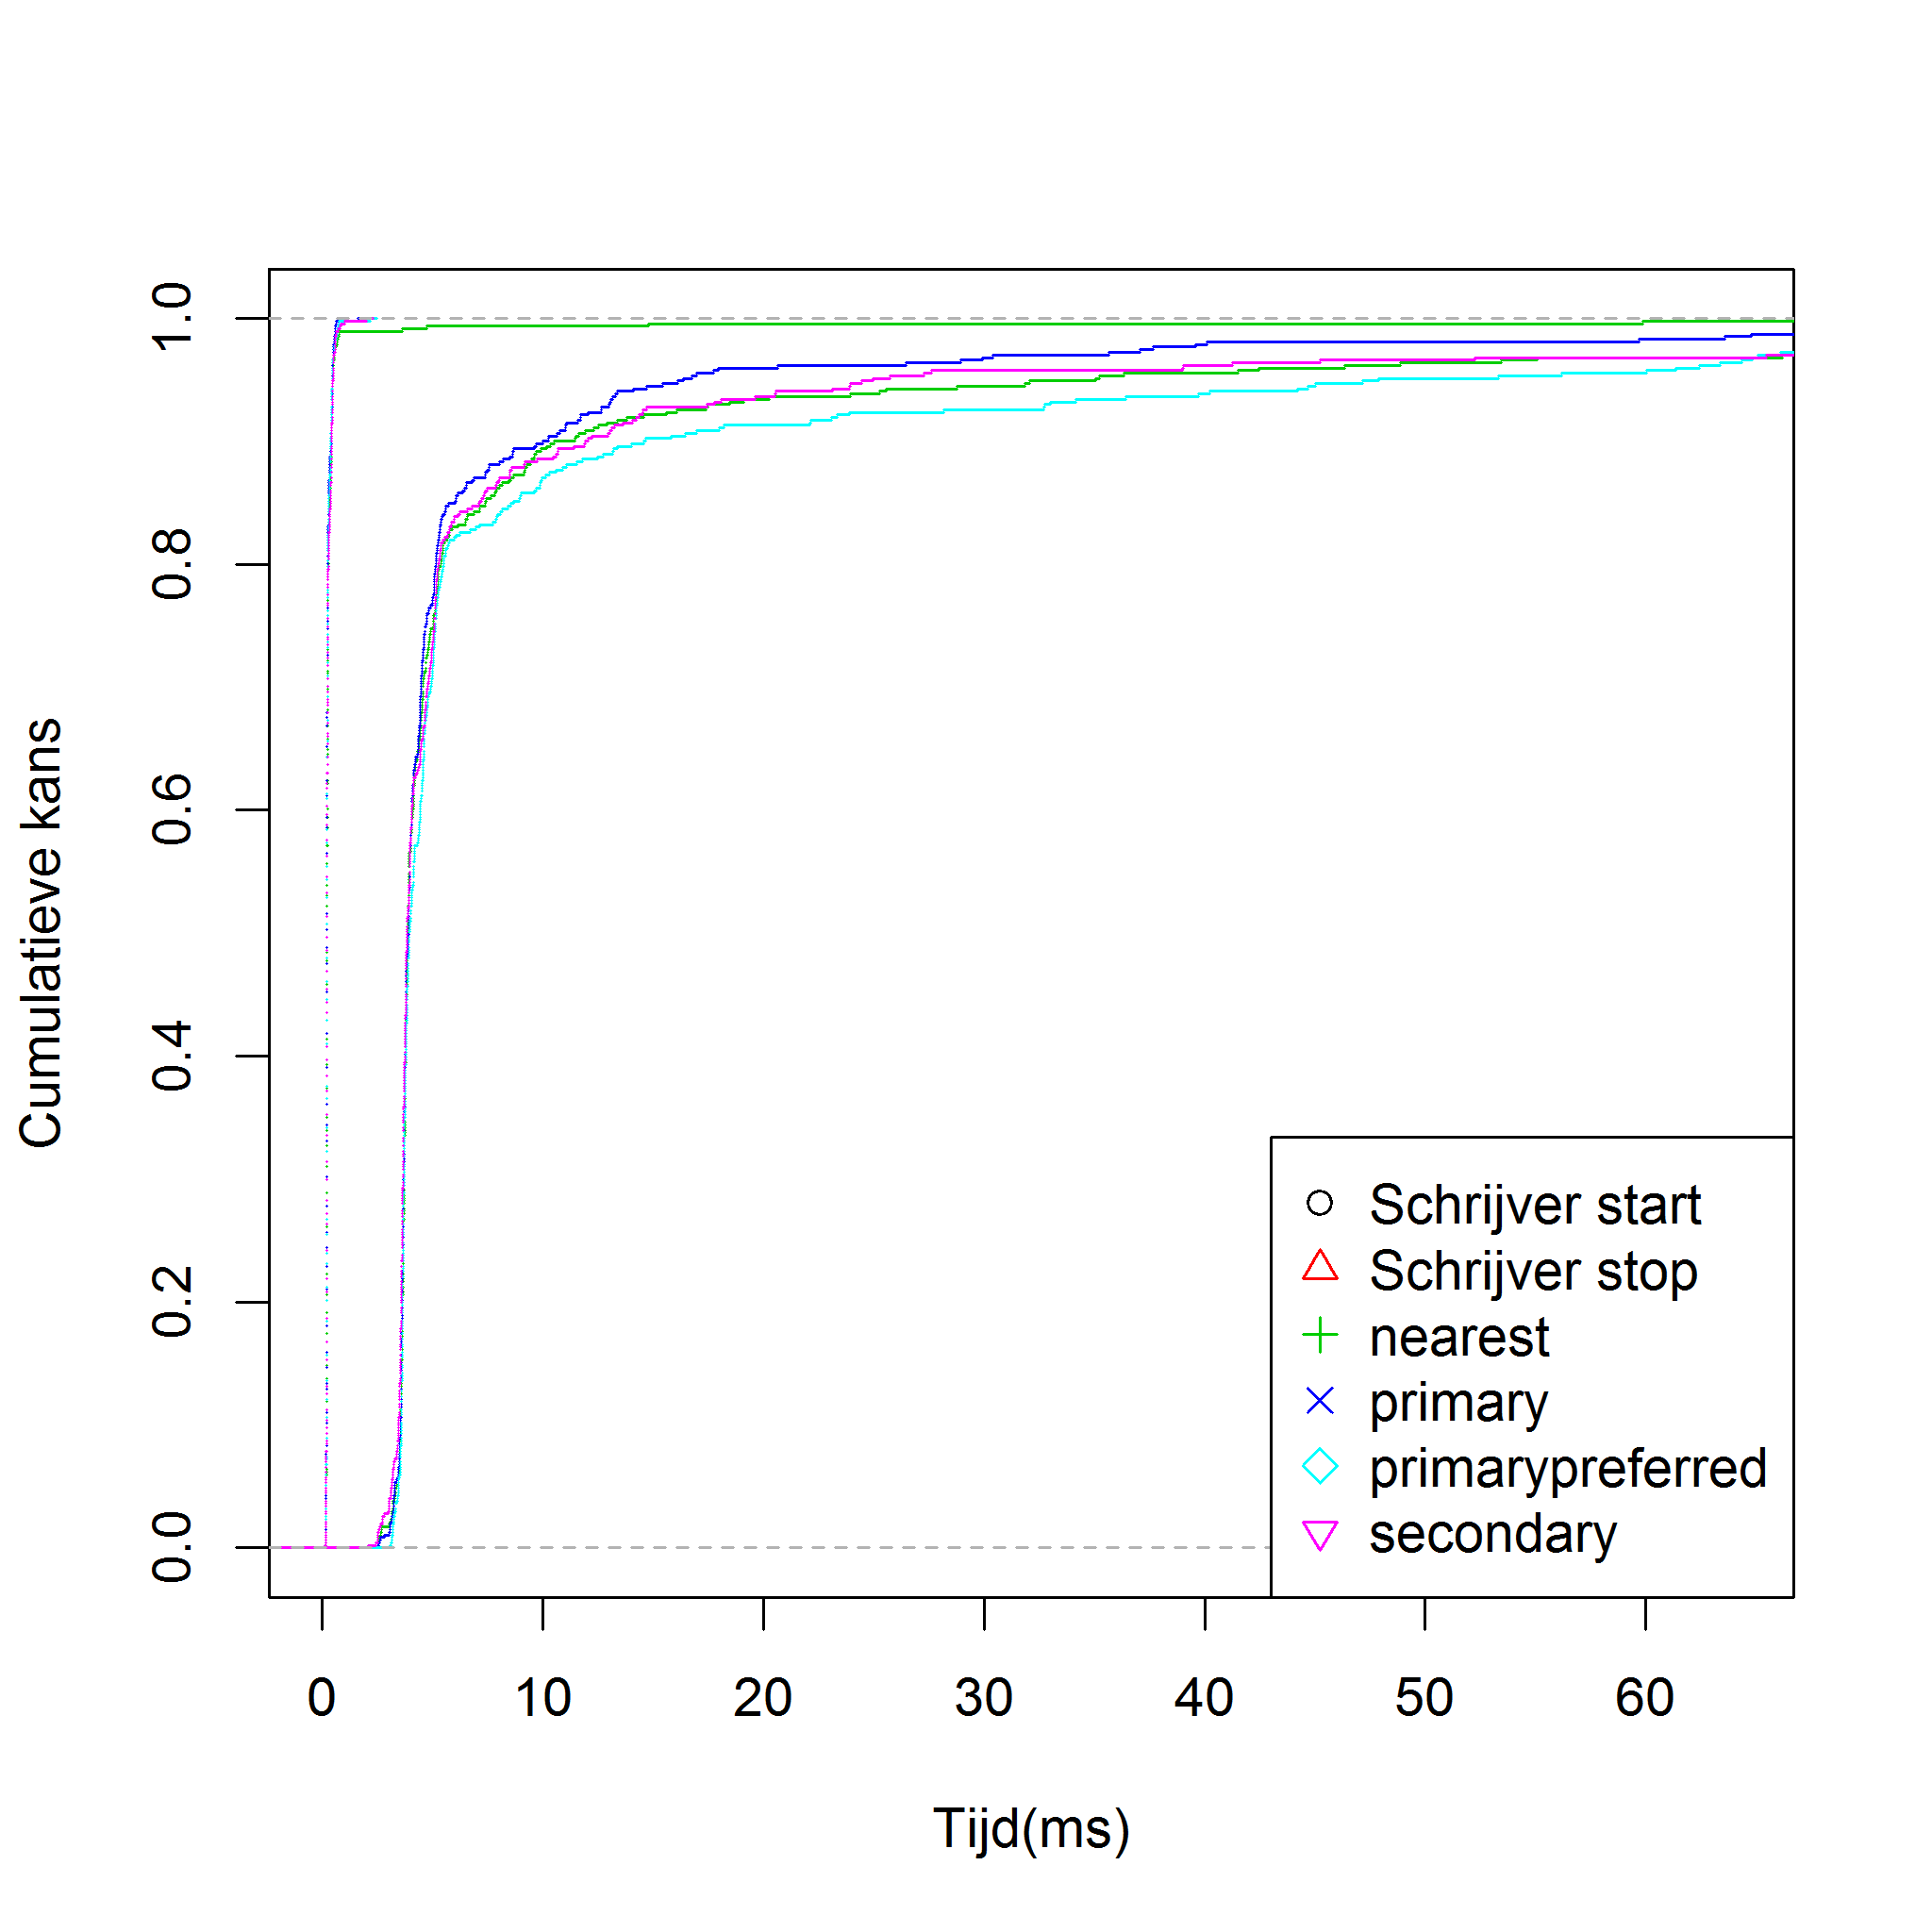
\includegraphics[width=.40\textwidth]{img/Observaties/MongoDB/ECDF-Reads-update-majority-1-2}}
%	\subfigure[Majority Insert]{\label{fig:consistentie-mongodb-R2-majority-insert} 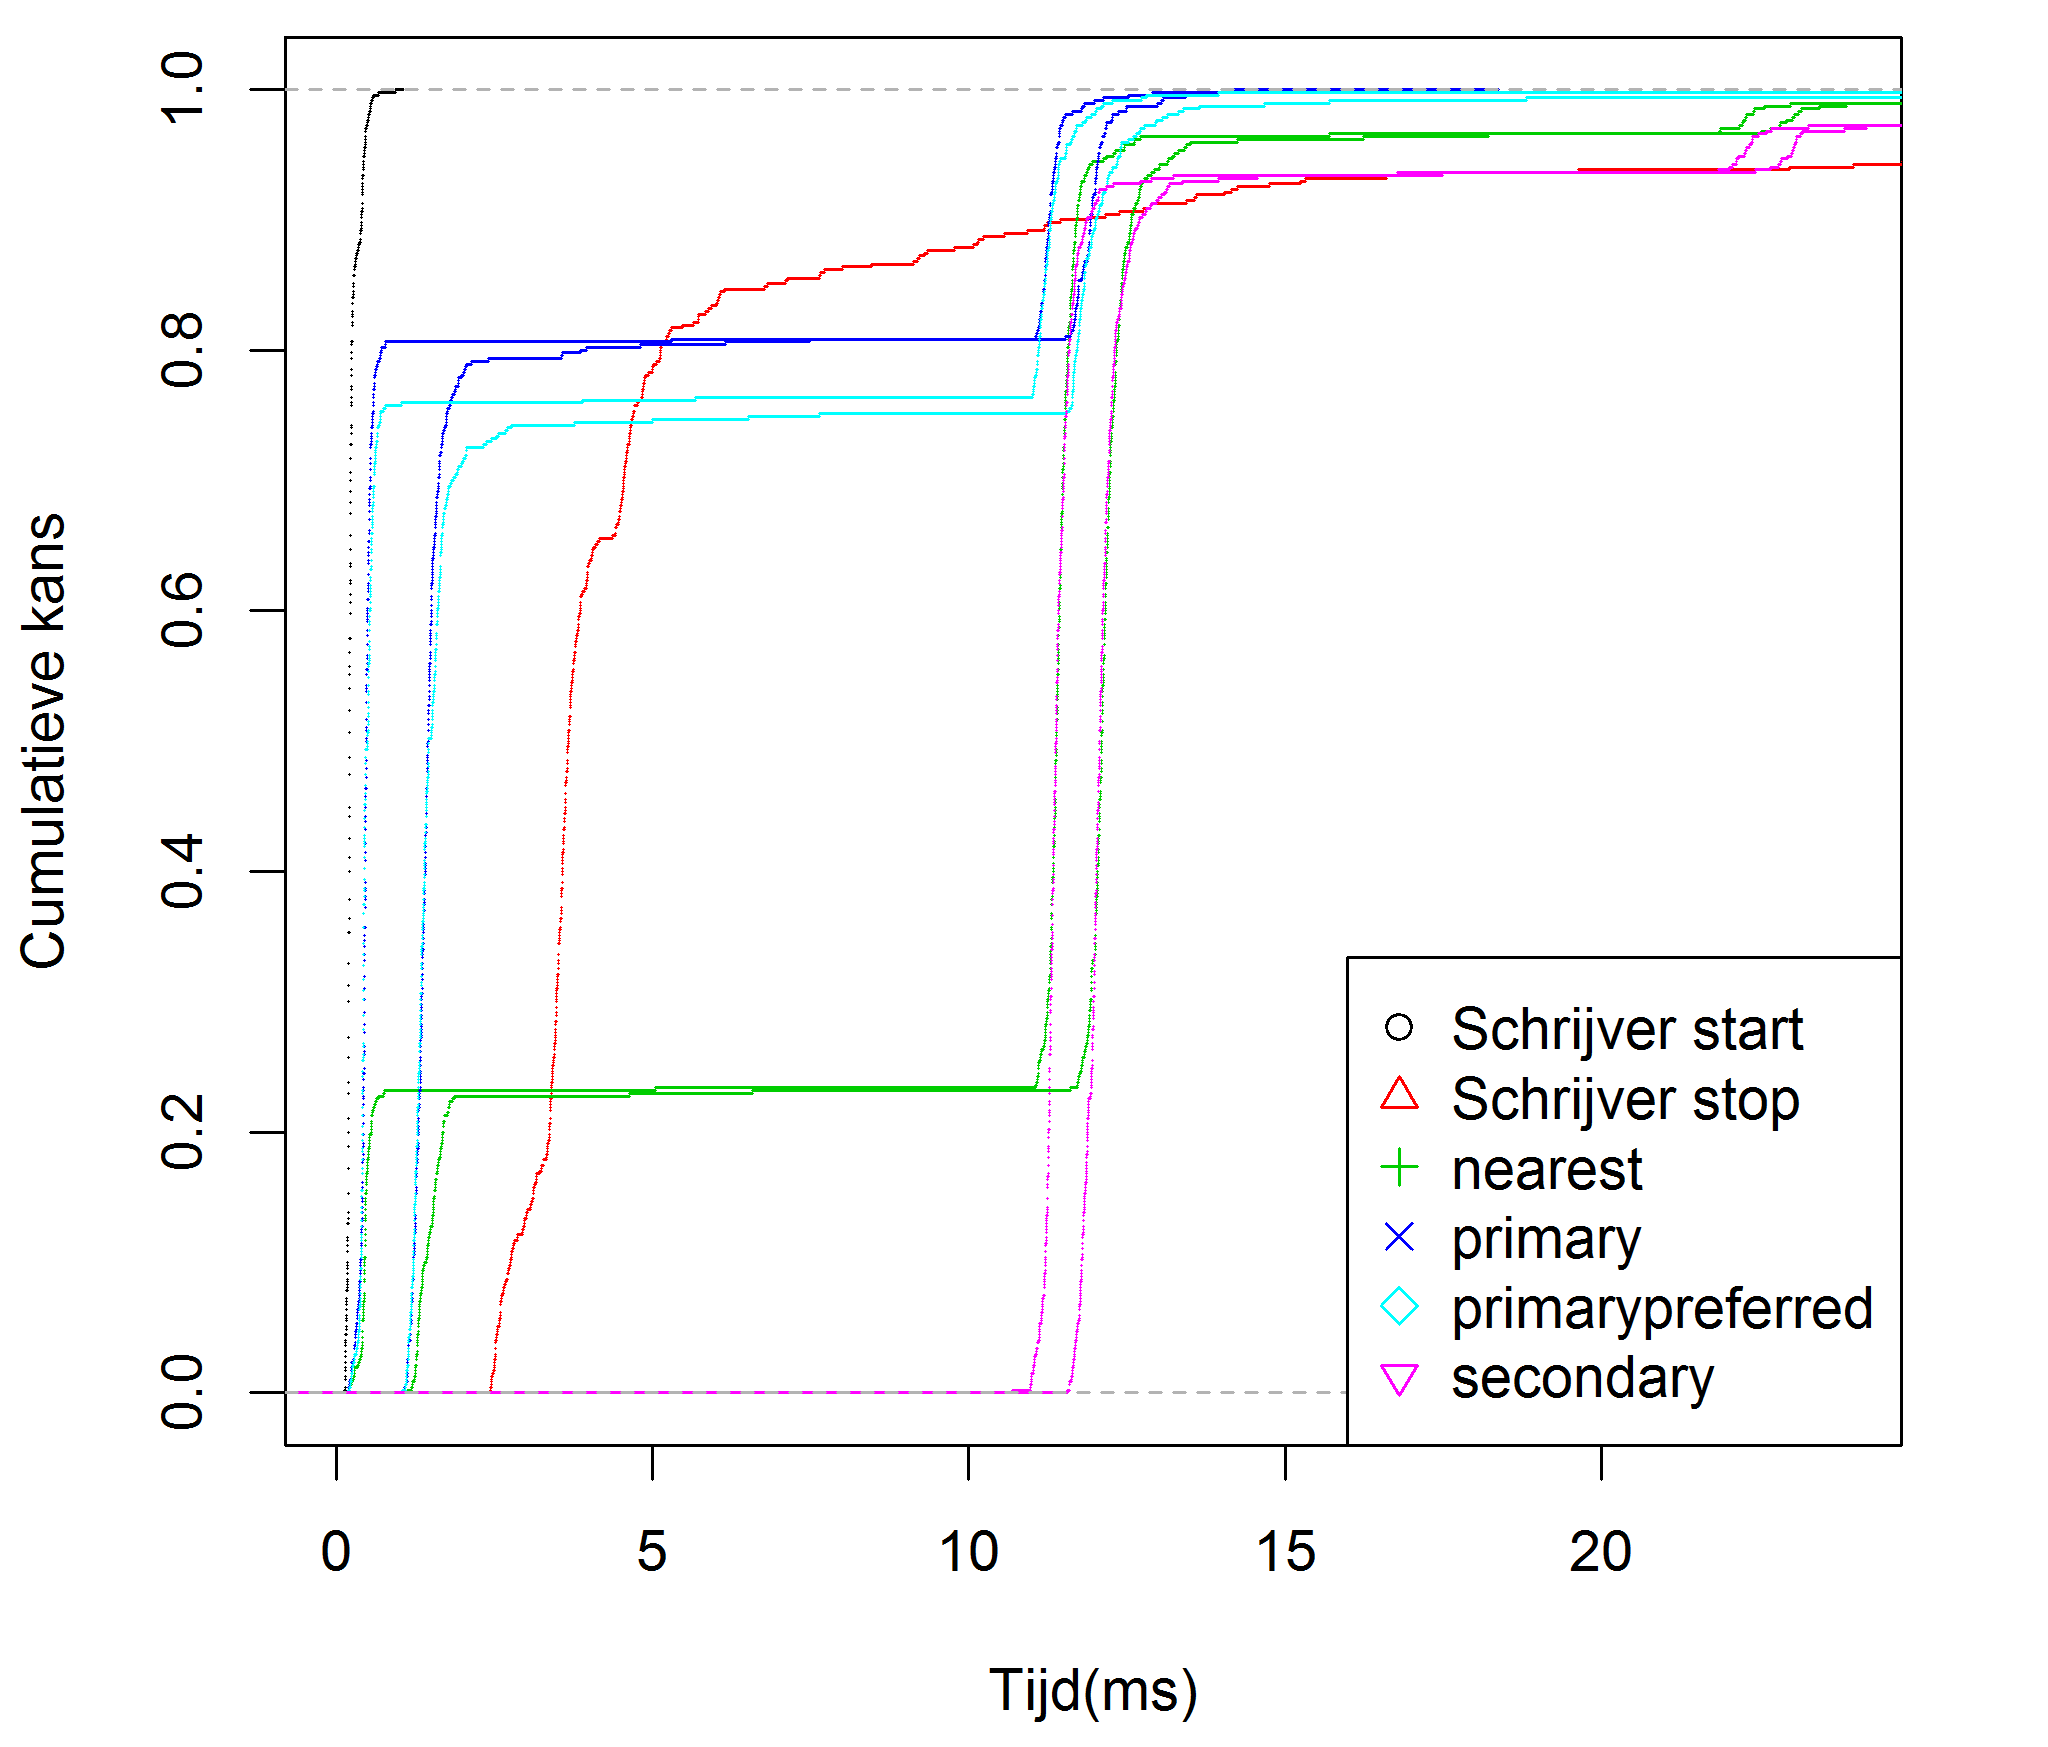
\includegraphics[width=.40\textwidth]{img/Observaties/MongoDB/ECDF-Reads-insert-majority-1-2}}
%	\caption{Consistentie: Overzicht van MongoDB op de consistentie testen voor lezer 2 met een 99-percentiel (voor de lezers) met start en stoptijden in dezelfde kleur.}
%	\label{fig:consistentie-mongodb-R2}
%\end{figure}
